\documentclass[12pt,spanish]{article}
\usepackage[spanish]{babel}
\usepackage{graphicx}
\usepackage{color}
\usepackage{xcolor}
\usepackage{colortbl}
\usepackage{amsthm,thmtools}
\usepackage{multirow}
\usepackage{amsmath}
\usepackage{subcaption}
\usepackage{adjustbox}
\usepackage{amsmath}
\usepackage{centernot}
\usepackage{multirow}
\usepackage[hidelinks]{hyperref}
\usepackage{caption}
\usepackage{eurosym} % para el euro
\usepackage{amsthm}
\usepackage{multicol}
\usepackage{float}
\usepackage{amsfonts}
\usepackage{titling}
\usepackage{soul}
\usepackage{listings}
\usepackage{array}
\usepackage{tikz}
\usetikzlibrary{shapes.geometric, arrows, chains, calc,positioning,fit,decorations.pathreplacing}
\usepackage[framemethod=tikz]{mdframed}

\graphicspath{ {../img/}}
\selectlanguage{spanish}
\usepackage[utf8]{inputenc}
\usepackage{graphicx}
\usepackage[a4paper,left=3cm,right=2cm,top=2.5cm,bottom=2.5cm]{geometry}

\newenvironment{solution}{
	\par
	\textbf{Solución}
	\par
	\begin{center}
}
{
	\end{center}
}


\title{Ingeniería de Servidores}
\setlength{\droptitle}{10em}
\author{Carlos Sánchez Páez}

\makeindex
\begin{document}
\definecolor{light-gray}{gray}{0.95}
\lstset{columns=fullflexible,basicstyle=\ttfamily}
\surroundwithmdframed[
  hidealllines=true,
  backgroundcolor=light-gray,
  innerleftmargin=0pt,
  innertopmargin=0pt,
  innerbottommargin=0pt]{lstlisting}


\begin{titlepage}

 \newlength{\centeroffset}
 \setlength{\centeroffset}{-0.5\oddsidemargin}
 \addtolength{\centeroffset}{0.5\evensidemargin}
 \thispagestyle{empty}

 \noindent\hspace*{\centeroffset}
 \begin{minipage}{\textwidth}

  \centering
  
\includegraphics[width=0.9\textwidth]{logo_ugr.jpg}\\[1.4cm]

  \textsc{ \Large Ingeniería de Servidores\\[0.2cm]}
  \textsc{GRADO EN INGENIERÍA INFORMÁTICA}\\[1cm]

  {\Huge\bfseries Resumen del temario\\}
 \end{minipage}

 \vspace{1.5cm}
 \noindent\hspace*{\centeroffset}
 \begin{minipage}{\textwidth}
  \centering

  \textbf{Autor}\\ {Carlos Sánchez Páez}\\[2.5ex]
  
\includegraphics[width=0.4\textwidth]{etsiit_logo.png}\\[0.1cm]
  \vspace{1.5cm}
  
\includegraphics[width=0.15\textwidth]{atc.jpg}\\[0.1cm]
  \vspace{1cm}
  \textsc{Escuela Técnica Superior de Ingenierías Informática y de Telecomunicación}\\
  \vspace{1cm}
  \textsc{Curso 2019-2020}
 \end{minipage}
\end{titlepage}
\thispagestyle{empty}
\newpage
\tableofcontents{}
\newpage
\listoffigures
\thispagestyle{empty}
\newpage

\section{Tema 1. Introducción a la Ingeniería de Servidores}

\subsection{¿Qué es un servidor?}

Un \textbf{sistema informático} es un conjunto de elementos \textit{hardware} (componentes físicos), \textit{software} (componentes lógicos) y \textit{peopleware} (recursos humanos) que permite obtener, procesar y almacenar información.\\
Los sistemas informáticos se pueden clasificar atendiendo a varios factores:
\begin{itemize}
	\item Según el nivel de paralelismo (\textit{SISD},\textit{SIMD},\textit{MISD} o \textit{MIMD})
	\item Según su uso (propósito general o específico)
	\item[*] Si son servidores, según la arquitectura de servicio (sistema aislado, cliente-servidor, \emph{n} capas o cliente-cola-cliente)
\end{itemize}

\subsubsection{Según su nivel de paralelismo}

\begin{itemize}
	\item \textit{SISD}: \textbf{S}ingle \textbf{I}nstruction \textbf{S}ingle \textbf{D}ata
	\item \textit{SIMD}: \textbf{S}ingle \textbf{I}nstruction \textbf{M}ultiple \textbf{D}ata
	\item \textit{MISD}: \textbf{M}ultiple \textbf{I}nstruction  \textbf{S}ingle \textbf{D}ata
	\item \textit{MIMD}: \textbf{M}ultiple \textbf{I}nstruction  \textbf{M}ultiple \textbf{D}ata
\end{itemize}
\begin{figure}[H]
	\centering
	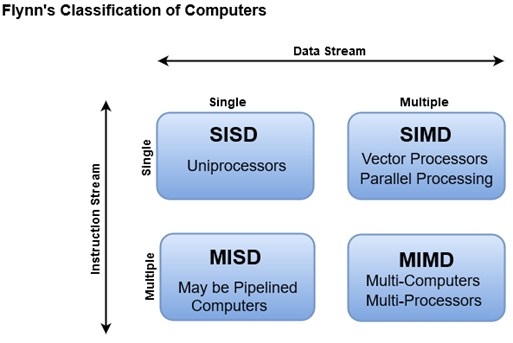
\includegraphics[width=0.5\textwidth]{comparacion_paralelismo.png}
	\caption{Sistemas informáticos según su nivel de paralelismo}
\end{figure}

\subsubsection{Según su uso}

\begin{itemize}
	\item De \textbf{uso general}: sirven para ejecutar diversas aplicaciones (PC sobremesa, portátil).
	\item De \textbf{uso específico}: ejecutan una función concreta.
	\begin{itemize}
		\item \textbf{Sistemas empotrados (\textit{embedded systems})}. Son sistemas acoplados a otro dispositivo o aparato que realizan una o varias funciones dedicadas. Suelen tener grandes restricciones de tamaño, tiempo de respuesta, etc. Suelen estar formados por un microprocesador, memoria y una amplia gama de interfaces de comunicación.Ejemplo: taxímetro, cámara de vigilancia, lavadora, etc.
		\item \textbf{Servidores}. Son sistemas informáticos que forman parte de una red y proporcionan servicios a otros sistemas informáticos (clientes). Puede ser cualquier computador o \textit{clúster} (agrupación de computadores que son percibidos externamente como uno solo).
	\end{itemize}
\end{itemize}

Hay varios tipos de servidores:
\begin{itemize}
	\item \textbf{Servidor de archivos}: permite el acceso remoto a archivos almacenados o directamente accesibles por él.
	\item \textbf{Servidor web}: almacena documentos HTML, imágines, etc. y distribuye el contenido a los clientes que lo soliciten.
	\item \textbf{Servidor de base de datos}: provee servicios de base de datos a otros programas o sistemas.
	\item \textbf{Servidor de \textit{e-commerce}}: cumple o procesa transacciones comerciales. Valida al cliente y genera un pedido al servidor de bases de datos.
	\item \textbf{Servidor de impresión}: controla una o más impresoras y acepta trabajos de impresión de los clientes de la red.
	\item \textbf{Servidor de correo electrónico}: almacena, envía, recibe, etc. correos electrónicos para los clientes de la red.
\end{itemize}

\subsubsection{Según su arquitectura de servicio}
\begin{itemize}
	\item \textbf{Sistema aislado}: es un sistema que no interactúa con otros. La arquitectura es monolítica y no se distribuye la información
	\item \textbf{Arquitectura cliente-servidor}: las tareas se reparten entre los servidores (reciben solicitudes) y los clientes (remiten solicitudes). Los nodos son los servidores y los clientes.
	\item \textbf{Arquitectura cliente-servidor de \emph{n} capas}: es una arquitectura cliente-servidor que tiene \emph{n} tipos de nodos en la red, por lo que se mejora la distribución de la carga (mejorando la escalabilidad). Sus principales puntos negativos son la sobrecarga de la red que conlleva y la dificultad de programación y administración.\\
	Ejemplo de arquitectura de 3 capas:
	\begin{enumerate}
		\item Servidores que interactúan con los clientes.
		\item Servidores de \textit{e-commerce} que procesan los datos para los servidores de la capa 1.
		\item Servidores de bases de datos que buscan, gestionan y almacenan los datos para los servidores de la capa 2.
	\end{enumerate}
	\item \textbf{Arquitectura cliente-cola-cliente}: el servidor únicamente pone en contacto a los clientes y sincroniza el sistema, mientras que los clientes se encargan de cooperar para realizar la función necesaria. La arquitectura \textit{P2P} está basada en este concepto. Ejemplos: \textit{Skype}, \textit{eMule}, \textit{BitTorrent}.
\end{itemize}

\subsection{Fundamentos de la Ingeniería de Servidores}

Un servidor se compone de:
\begin{itemize}
	\item Recursos físicos (placa base, memoria, CPU, etc.).
	\item Recursos lógicos (sistema operativo, aplicaciones).
	\item Recursos humanos (administración).
	\item Requisitos funcionales (prestaciones, seguridad, mantenimiento, disponibilidad, extensibilidad, escalabilidad, coste, fiabilidad...)
\end{itemize}

Las \textbf{prestaciones} cuantifican la velocidad con la que se realiza una determinada cantidad de trabajo o carga (\textit{workload}). Aquel servidor que realiza la misma carga de trabajo en menor tiempo es el que mayores prestaciones tiene.\\
Las medidas fundamentales para medir las prestaciones de un servidor son:
\begin{itemize}
	\item \textbf{Tiempo de respuesta} o \textbf{latencia}. Tiempo desde que se solicita una tarea al servidor hasta que finaliza. Por ejemplo: tiempo de ejecución de un programa, de acceso al disco, etc.
	\item \textbf{Productividad} (\textit{throughput}) o \textbf{ancho de banda} (\textit{bandwidth}). Cantidad de trabajo realizado por el servidor por unidad de tiempo. Por ejemplo: programas ejecutados por hora o páginas por hora servidas en el caso de un servidor web.
\end{itemize}

Los principales elementos que afectan a las prestaciones de un servidor son los siguientes:
\begin{itemize}
	\item Hardware del sistema (características y configuración).
	\item Parámetros del sistema operativo (configuración de memoria virtual, políticas de planificación...) y diseño de los programas (acceso a E/S, fallos de caché...).
	\item Actualización de componentes (reemplazar por dispositivos más rápidos) y configuración de dispositivos.
	\item Ajuste o sintonización del SO y los programas.
	\item Distribución de carga (\textit{load balancing}): dar mayor carga a los dispositivos más rápidos.
\end{itemize}

\subsubsection{Requisitos funcionales de un servidor}

\begin{itemize}
	\item \textbf{Disponibilidad} (\textit{Availability}). Un servidor está disponible si está en estado operativo.\\ El tiempo de inactividad (\textit{downtime}) es la cantidad de tiempo en la que el sistema no está disponible. Puede ser de dos tipos:
	\begin{itemize}
		\item Planificado (actualizaciones de hardware o software que no se puedan realizar en caliente).
		\item No planificado (a causa de algún fallo).
		
		\rightarrow Si el sistema tiene \emph{alta disponibilidad} será \emph{tolerante a fallos}.
	\end{itemize}
	\newpage
	Algunas soluciones para aumentar la disponibilidad son:
	\begin{itemize}
		\item Reemplazo en caliente de los componentes (\textit{hot-swapping}).
		\item Sistemas redundantes de discos (\textit{RAID}), alimentación y red.
		\item Sistemas distribuidos.
	\end{itemize}
	\item \textbf{Fiabilidad} (\textit{Reliability}). Un sistema es fiable cuando realiza su actividad sin errores. Se aplica más a componentes por separado. El \textbf{MTTF} (\textit{\textbf{M}ean \textbf{T}ime \textbf{T}o \textbf{F}ailure}) es el tiempo medio que tiene un sistema hasta que ocurre un error. Los mecanismos para asegurar la fiablilidad son la comprobación (\textit{checksums}, bits de paridad, etc.)
	\item \textbf{Seguridad}. Un servidor debe ser seguro ante:
	\begin{itemize}
		\item La incursión de individuos no autorizados (\textit{confidencialidad}).
		\item La corrupción o alteración no autorizada de datos (\textit{integridad}).
		\item Las interferencias (ataques) que impidan el acceso a los recursos.
	\end{itemize}
	Las principales soluciones son la encriptación de datos, el uso de cortafuegos y la autenticación segura de usuarios.
	\item \textbf{Extensibilidad-expansibilidad}. Es la facilidad que ofrece el sistema para aumentar sus características o recursos (tener bahías libres para discos duros o memoria, uso de sistemas operativos modulares, uso de interfaces de entrada y salida estándar, etc.). Cualquier solución que facilite la escalabilidad facilita también la extensibilidad.
	\item \textbf{Escalabilidad}. Un servidor es escalable si sus prestaciones pueden aumentar significativamente ante un incremento significativo de la carga. Las soluciones más usadas son la virtualización, la programación paralela y la tecnología \textit{cloud}. Todos los sistemas escalables son extensibles (pero no al revés).
	\item \textbf{Mantenimiento}. Son las acciones que sirven para prolongar el funcionamiento correcto del sistema. Es importante que el servidor sea fácil de mantener (sistema operativo actualizado, garantía de componentes, copias de seguridad, etc.).
	\item \textbf{Coste}. Debemos escoger un diseño que sea asequible y se ajuste al presupuesto teniendo en cuenta el coste hardware, software, de actualizaciones, de personal, de proveedores de red, de alquiler de local y de \textbf{eficiencia energética}. La eficiencia energética es clave ya que reduce en gran cantidad los costes (consumo de potencia, refrigeración) y además ayuda a preservar el medio ambiente. Las soluciones más comunes son:
	\begin{itemize}
		\item Ajuste automático de potencia de los componentes según la carga.
		\item \textit{Free cooling}, aprovechamiento de las bajas temperaturas exteriores para tener refrigeración gratuita.
		\item Fusionar varios servidores con poco uso en un único servidor.
	\end{itemize}

\end{itemize}

\subsection{Comparación conjunta entre prestaciones y coste}

El computador de mejores prestaciones (el más rápido) para un determinado conjunto de programas será el que lo ejecute en menor tiempo.\\

\subsubsection{Tiempos de ejecución mayores o menores}

Sea $t_A$ el tiempo de ejecución de un programa en la máquina A (ídem para $t_B$).
\begin{itemize}
	\item $t_A$ es $\frac{t_A}{t_B}$ veces $t_B$. Por ejemplo, si $t_A=10s$ y $t_B=5s$, $t_A$ es $\frac{10}{5}=2$ veces $t_B$ (el doble).
	\item Igualmente, $t_B$ es $\frac{5}{10}=0.5$ veces $t_A$ (la mitad).
\end{itemize}

El \textbf{cambio relativo de $t_A$ con respecto a $t_B$}; $\Delta t_{A,B}(\%)$ viene dado por:
\[
t_A=t_B + \frac{\Delta t_{A,B}(\%)}{100} * t_B
\]
Es decir, es el porcentaje que le falta a $t_B$ para ser $t_A$.\\
En el ejemplo anterior el cambio relativo de $t_A$ con respecto a $t_B$ es del 100\%. Es decir, a $t_B$ le falta un 100\% de sí mismo (el doble) para llegar a ser $t_A$.\\
De igual forma, el cambio relativo de $t_B$ con respecto a $t_A$ es del -50\% (a $t_A$ le sobra la mitad para ser $t_B$).\\
Usando el lenguaje común podríamos traducir los resultados en:
\begin{itemize}
	\item $t_A$ es un 100\% mayor que $t_B$ y $t_B$ es un 50\% menor que $t_A$.
	\item $t_A$ es 2 veces mayor que $t_B$ (¡ojo! ¡¡"1 vez mayor" significa igual!!).
\end{itemize}

La velocidad de ejecución de una máquina será inversamente proporcional al tiempo que tarda en ejecutarse. Teniendo ésto en cuenta podemos definir la aceleración (\textit{speedup}) de A con respecto a B de la siguiente forma:
\[
S_B(A)=\frac{v_A}{v_B}=\frac{t_B}{t_A}
\]
El cambio relativo de $v_A$ con respecto de $v_B$ (es decir, el porcentaje de cambio en velocidad al reemplazar A por B) viene dado por:
\[
\Delta v_{A,B}(\%)=(S_B(A) -1) * 100
\]

Supongamos que para un programa, $t_A=36s$ y $t_B=45s$.\\
La ganancia de velocidad de A con respecto a B sería:
\[
S_B(A)=\frac{v_A}{v_B}=\frac{t_B}{t_A}=\frac{45 s}{36 s}=1.25
\]
El cambio relativo de $v_A$ con respecto a $v_B$ (es decir, el porcentaje de mejora) viene dado por:
\[
\Delta v_{A,B}(\%)=(S_B(A)-1) * 100 = (1.25 - 1) * 100 = 0.25 * 100 = 25\%
\]
Usando el lenguaje común diríamos que:
\begin{itemize}
	\item A es 1.25 veces más rápida que B.
	\item A es un 25\% más rápida que B
\end{itemize}
De igual forma:
\[
S_A(B)=\frac{t_A}{t_B}=\frac{36 s}{45 s}=0.8
\]
\[
\Delta v_{B,A}(\%)=(S_A(B)-1) * 100 = (0.8 - 1) * 100 = -0.2 * 100 = -20\%
\]
Es decir, B es un 20\% más lenta que A.

\begin{center}
	¡¡Ojo!! \\
	A es un $x\%$ más rápida que B $\centernot\implies$ B es un $x\%$ más lenta que A.\\
	Por ejemplo, 10 es un 100\% mayor que 5 $\centernot\implies$ 5 es un 100\% menor que 10
\end{center}

Supongamos que en el ejemplo anterior el computador A cuesta 625 \textup{\euro} y el computador B, 550 \textup{\euro}.
\begin{itemize}
	\item A es $\frac{625}{550}=1.14$ veces más caro que B (un 14\% más caro).
	\item ¿Cuál ofrece mejor relación prestaciones/precio para nuestro programa?
	\[
		\frac{Prestaciones_A}{Coste_A}=\frac{v_A}{Coste_A} \propto \frac{\frac{1}{t_A}}{Coste_A}=\frac{\frac{1}{36 s}}{625 \textup{\euro}} = 4.4 * 10^{-5} \frac{s^{-1}}{\textup{\euro}}
	\]

	\[
		\frac{Prestaciones_B}{Coste_B}=\frac{v_B}{Coste_B} \propto \frac{\frac{1}{t_B}}{Coste_B}=\frac{\frac{1}{45 s}}{550 \textup{\euro}} = 4.0 * 10^{-5} \frac{s^{-1}}{\textup{\euro}}
	\]
	Pasamos ahora a comparar ambas relaciones:
	\[
	\frac{\frac{Prestaciones_A}{Coste_A}}{\frac{Prestaciones_B}{Coste_B}} = \frac{4.4 * 10^{-5}}{4.0 * 10^{-5}} = 1.1
	\]
	\item Por tanto, el computador A presenta una mayor relación prestaciones/coste que B (un 1.1 mayor $=$ un 10\% mayor) para nuestro programa.
\end{itemize}


\subsection{Límites en la mejora del tiempo de respuesta}

La mejora dekl tiempo de respuesta no es ilimitada, por lo que debemos saber hacia dónde dirigir los esfuerzos. Por ejemplo, si un programa utiliza la CPU en un 80\% del tiempo y la impresora en un 20\% debemos centrarnos en mejorar la CPU. El planteamiento sería el siguiente:
\begin{itemize}
	\item Un sistema tarda un tiempo $T_{original}$ en ejecutar un programa monohebra.
	\item Mejoramos el sistema reemplazando un componente por otro $k$ veces más rápido.
	\item Este comonente se utilizaba durante una fracción $f$ de $T_{original}$ (si $f=1$, el componente se utilizaba el 100\% del tiempo).
	\item ¿Qué ganancia en prestaciones (\textit{speedup}) hemos conseguido con el cambio?
\end{itemize}
\newpage
\begin{figure}[H]
	\centering
	\begin{tikzpicture}[arrow/.style = {thick,-stealth}]
		\tikzset{set/.style={draw,rectangle,inner sep=0pt,align=center}}
		\node[fit={(0,0) (5,1.5)}, inner sep=0pt, draw=black, thick, fill=blue!20, text centered] (nousado1) { Recurso no utilizado \\($1-f * t_O$)};
		\node[fit={(5,0) (15,1.5)}, inner sep=0pt, draw=black, thick, fill=green!20, text centered] (usado1) {Recurso utilizado ($f * t_O$)};

		\node[fit={(0,-5) (5,-3.5)}, inner sep=0pt, draw=black, thick, fill=blue!20, text centered] (nousado2) { Recurso no utilizado \\($1-f * t_O$)};
		\node[fit={(5,-5) (10,-3.5)}, inner sep=0pt, draw=black, thick, fill=yellow!20, text centered] (usado2) {Recurso utilizado ($\frac{f * t_O}{k}$)};

		\draw [arrow] (5,0) -- (5,-3.5);
		\draw [arrow] (15,0) -- node [below right] {$k$ veces más pequeño} (10,-3.5);

		\draw [decorate,decoration={brace,amplitude=10pt, raise=2.5pt}]	(0,1.5) -- (15,1.5) node [black, midway, sloped, above=0.5cm] {Tiempo original $t_O$};

		\draw [decorate,decoration={brace,amplitude=10pt, raise=2.5pt, mirror}]	(0,-5) -- (10,-5) node [black, midway, sloped, below=0.5cm] {Tiempo mejorado $t_M$};

	\end{tikzpicture}
	\caption{Tiempos original y mejorado}
\end{figure}

\subsubsection{Ley de Amdahl}
¿Cuál es la ganancia en velocidad ($S$) del sistema después de mejorar $k$ veces un componente?
\begin{figure}[H]
	\begin{equation}
		S=\frac{1}{1-f+\frac{f}{k}}
	\end{equation}
	\caption{Ley de Amdahl}
\end{figure}
Donde:
\begin{itemize}
	\item Si $f=0 \implies S=1$, por lo que no hay mejora en el sistema (el recurso no se usaba).
	\item Si $f=1 \implies S=k$, el sistema mejora tantas veces como el componente (se usa siempre).
	\item Si $f\to \infty \implies S \to \lim_{k \to \infty} S=\frac{1}{1-f}$
\end{itemize}

Veamos un ejemplo:\\
La utilziación de un disco duro es del 60\% para un programa monohebra. ¿Cuál será la velocidad de ejecución si duplicamos la velocidad del disco?
\[
S=\frac{1}{1-f+\frac{f}{k}} \implies S=\frac{1}{1-0.6+\frac{0.6}{2}}=1.43
\]
Por tanto, el sistema es $1.43$ veces más rápido (un 43\% más rápido que antes).\\
Si sólo nos centráramos en mejorar el disco, la ganancia máxima que podríamos obtener sería:
\[
S_{max}=\lim_{k \to \infty}S=\frac{1}{1-f}=\frac{1}{1-0.6}=2.5
\]
Es decir, el sistema podría llegar a ser $2.5$ veces más rápido (un 150\% más rápido) que antes si sólo mejoramos el disco.

\subsubsection{Generalización de la ley de Amdahl}

Para $n$ mejoras, el \textit{speedup} vendría dado por:

\[
S=\frac{1}{(1-\sum_{i=1}^{n}f_i) + \sum_{i=1}^{n}\frac{f_i}{k_i}}
\]

También podemos calcular la aceleración con una sola mejora en cascada, teniendo en cuenta que debemos recalcular $f$ en cada paso. Sin embargo, es mucho más sencillo aplicar el procedimiento del \hyperref[1.13]{\textbf{ejercicio 1.3}}.
\newpage
\section{Tema 2. Componentes hardware de un servidor}

\subsection{Placa base (\textit{Motherboard})}
Es la tarjeta de circuito impreso (\textit{PCB}) que interconecta los distintos componentes.
\begin{figure}[H]
	\centering
	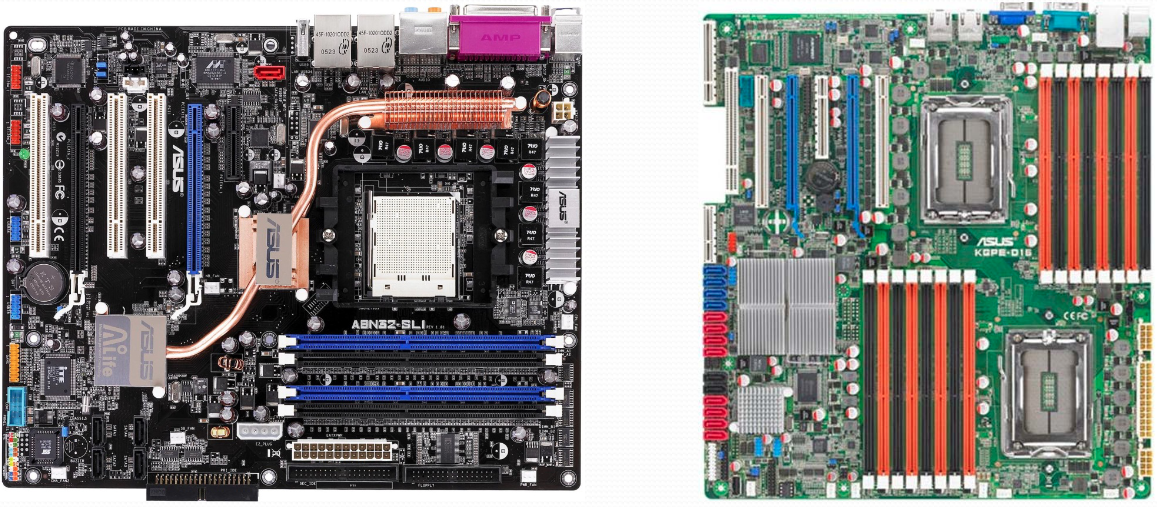
\includegraphics[width=0.5\textwidth]{mobos.png}
	\caption{Dos placas base}
\end{figure}
\subsubsection{Tarjeta de cirtuito impreso}

Está hecha de pistas de cobre rodeadas de un elemento aislante (fibra de vidrio con resina no inflamable).\\
Actualmente, las placas base son multi-capa. A través de unos agujeros (vías) se realiza la conexión de una capa con otra.\\
Las placas base tienen un tamaño (\textit{form factor}) estandarizado: \textit{Standard-ATX}, \textit{Micro-ATX}, \textit{Mini-ITX}...
\begin{figure}[H]
	\centering
	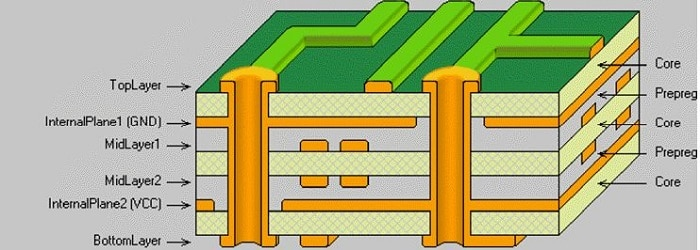
\includegraphics[width=0.5\textwidth]{pcb.jpg}
	\caption{\textit{PCB} multicapa}
\end{figure}

\begin{figure}[H]
	\centering
	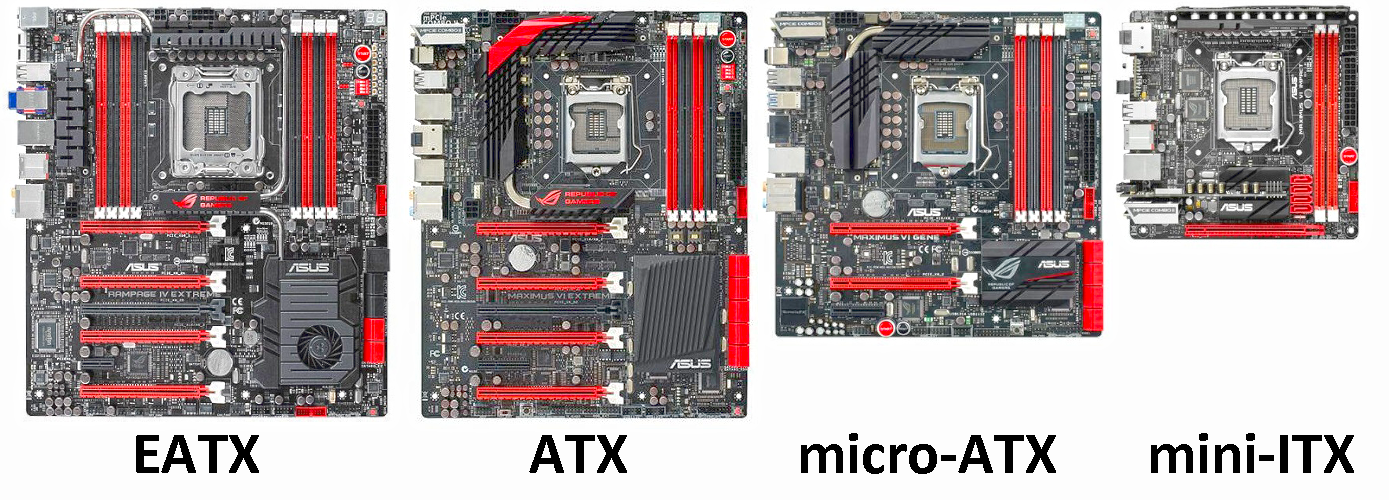
\includegraphics[width=0.5\textwidth]{moboformfactor.png}
	\caption{Distintos factores de forma de placas base}
\end{figure}

\subsubsection{Componentes de una placa base}
\begin{figure}[H]
	\centering
	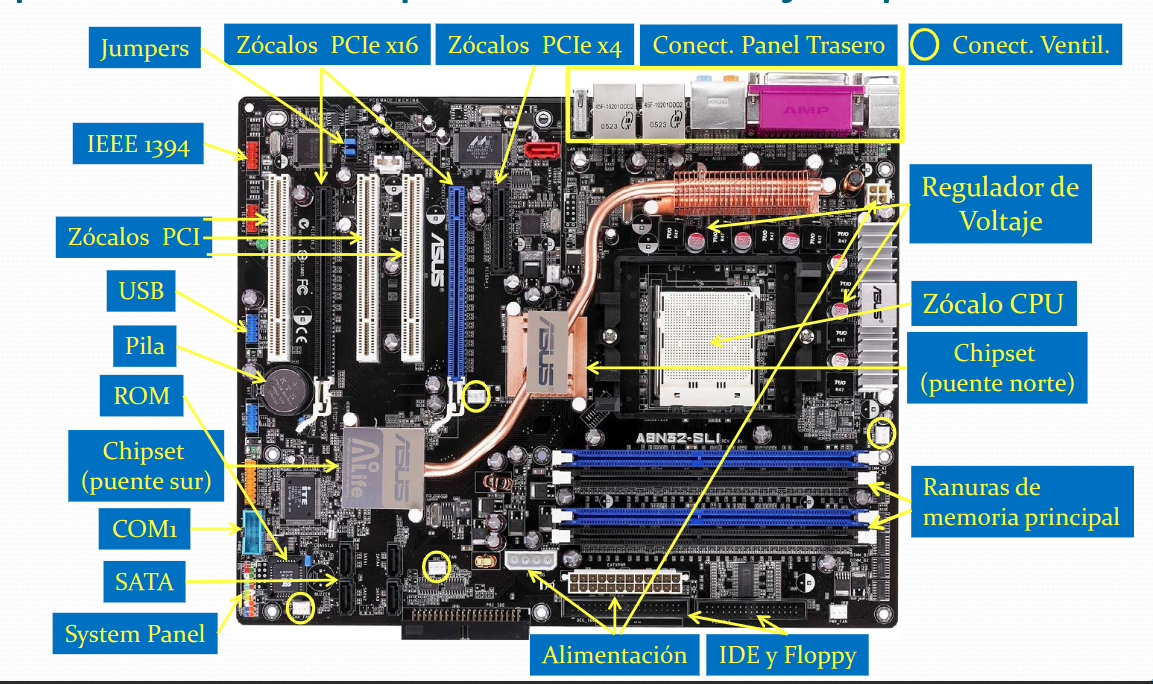
\includegraphics[width=\textwidth]{mobocomponents.png}
	\caption{Componentes de una placa base}
\end{figure}
En el manual de la placa podremos ver un esquema simple de la localización de sus principales componentes:

\begin{figure}[H]
	\centering
	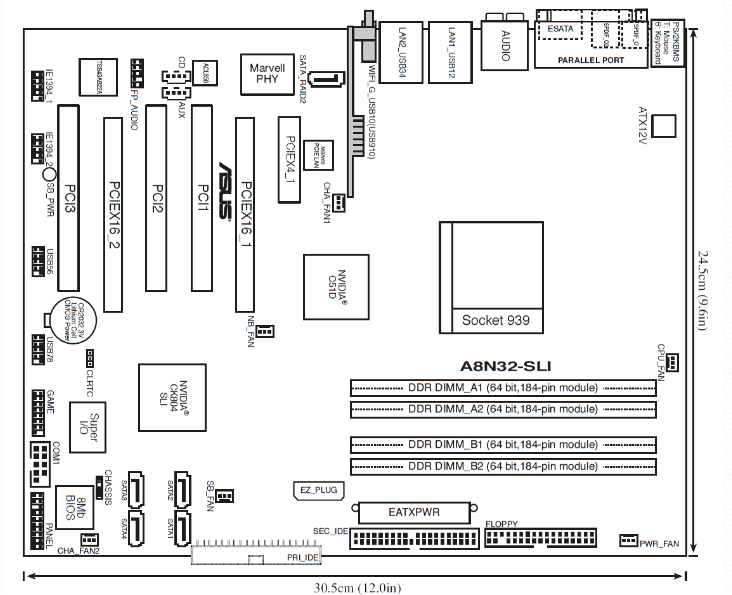
\includegraphics[width=0.75\textwidth]{mobocomponentsmanual.png}
	\caption{Esquema de componentes de una placa base según el manual}
\end{figure}

\subsubsection{Montaje de los componentes de una placa base}

Debemos tener mucho cuidado con la \textit{electricidad estática} de nuestro cuerpo. Si tenemos el cuerpo cargado y tocamos un elemento hardware podemos cortocircuitarlo y dañarlo. Para ello existen soluciones como descargar nuestro cuerpo tocando una gran superficie metálica o utilizar una pulsera de descarga (\textit{ESD, \textbf{E}lectro\textbf{S}tatic \textbf{D}ischarge}).

\begin{figure}[H]
	\centering
	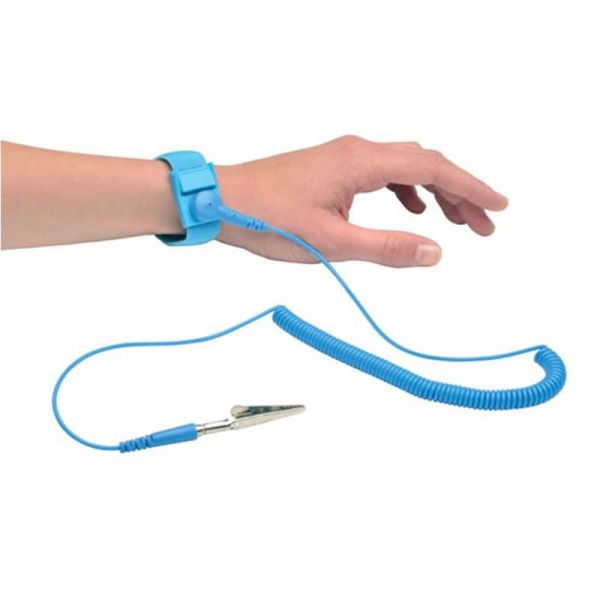
\includegraphics[width=0.35\textwidth]{esd.jpg}
	\caption{Pulsera de descarga}
\end{figure}
También es importante que manipulemos la máquina una vez que lleve un tiempo desenchufada. De esta forma, los condensadores se descargarán.

\subsection{Fuente de alimentación}
Se encarga de convertir la corriente alterna en continua.
\begin{itemize}
	\item Entrada: AC (220V-50Hz)
	\item Salida: DC($\pm$5V, $\pm$12V, $\pm$3.3V)
\end{itemize}
La fuente de alimentación (\textit{PSU, \textbf{P}ower \textbf{S}upply \textbf{U}nit}) alimenta tanto la placa base como los periféricos. Su factor más importante es la potencia que entrega (250W, 500W...)
\begin{figure}[H]
	\centering
	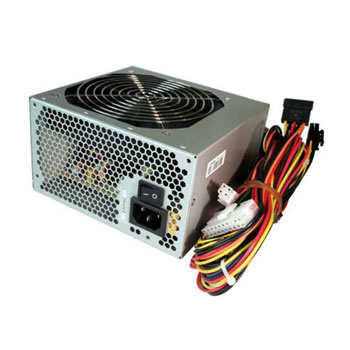
\includegraphics[width=0.35\textwidth]{psu.jpg}
	\caption{Fuente de alimentación}
\end{figure}

El voltaje $+5$V se utiliza normalmente cuando la máquina está en \textit{standby} para funciones como \textit{Wake On Lan} (encender cuando se solicite desde LAN).\\

Los distintos elementos de un ordenador (por ejemplo la CPU) necesitan a veces un voltaje menor (por ejemplo, 0.8V). Para ello existe el \textit{VRM, \textbf{V}oltage \textbf{R}egulation \textbf{M}odule} o módulo regulador de voltaje. Está compuesto por bovinas, condensadores y transistores y su misión es proporcionar corriente continua de distintos voltajes a los componentes y \textbf{mantenerla}, lo que aporta estabilidad. Suele colocarse cerca de los elementos que alimenta, como la CPU o la RAM. En equipos modernos se ubica bajo un disipador.

\begin{figure}[H]
	\centering
	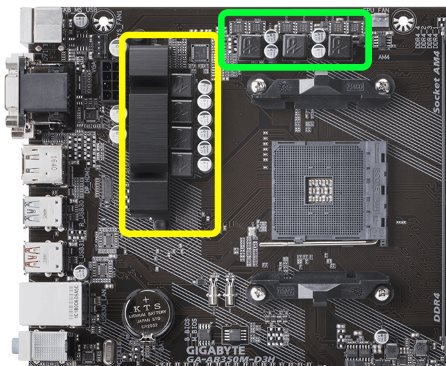
\includegraphics[width=0.35\textwidth]{vrm.jpg}
	\caption{Módulo de regulación de voltaje situado al lado del zócalo de la CPU}
\end{figure}

\begin{figure}[H]
	\centering
	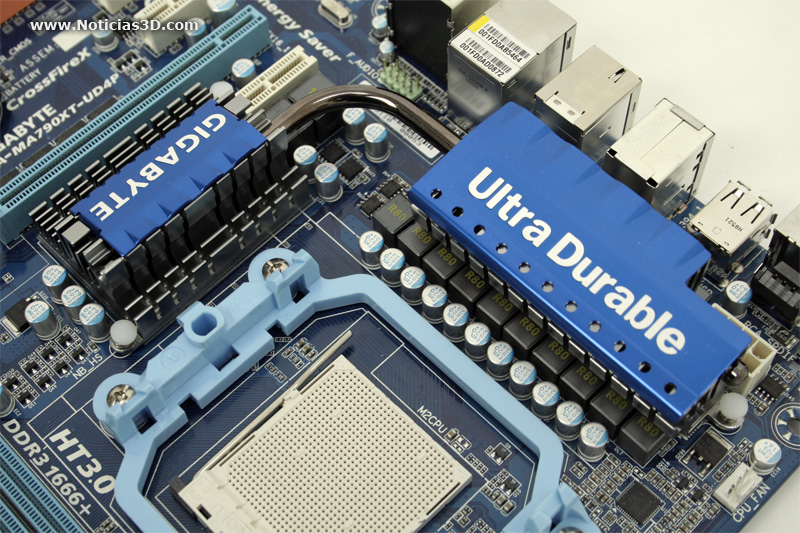
\includegraphics[width=0.35\textwidth]{vrm_disip.jpg}
	\caption{Módulo de regulación de voltaje bajo disipador}
\end{figure}

\subsection{Disipadores de calor}
Son elementos que se utilizan para bajar la temperatura de un componente. Transfieren el calor desde el componente hacia el aire. Pueden ser de dos tipos:
\begin{itemize}
	\item Pasivo (no necesita energía para funcionar).

	\item Activo (necesita energía, normalmente para un ventilador).
\end{itemize}
\begin{figure}[H]
	\centering
	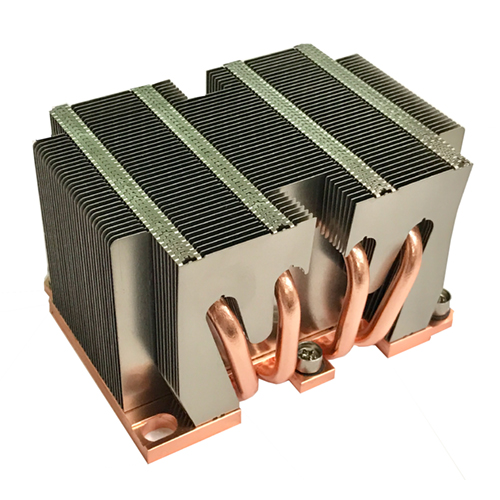
\includegraphics[width=0.25\textwidth]{passive.jpg}
	\caption{Disipador pasivo}
\end{figure}

\begin{figure}[H]
	\centering
	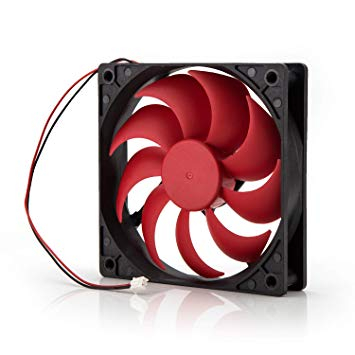
\includegraphics[width=0.25\textwidth]{fan.jpg}
	\caption{Disipador activo (ventilador de chasis)}
\end{figure}

Para refrigerar la CPU se combinan ambos tipos (a un disipador pasivo se le añade un ventilador). Este ventilador es controlado mediante un conector de 4 pines (\textit{CPU\_FAN}), que permite, además de darle energía al ventilador, controlar y medir su velocidad en cada momnento.\\

Para facilitar la transferencia de calor entre la CPU y el disipador pasivo se emplea \textit{pasta térmica}.

\begin{figure}[H]
	\centering
	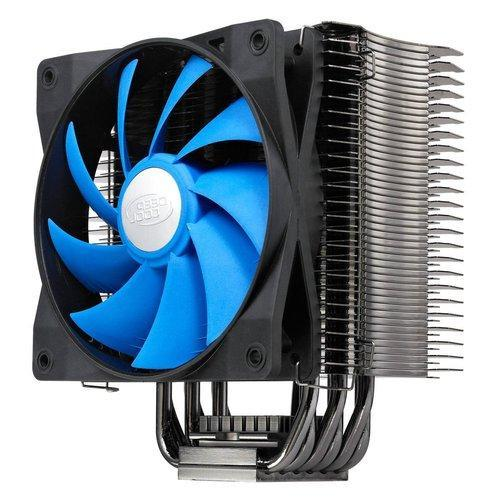
\includegraphics[width=0.25\textwidth]{cpufan.jpg}
	\caption{Disipador de CPU (combina activo y pasivo)}
\end{figure}

\begin{figure}[H]
	\centering
	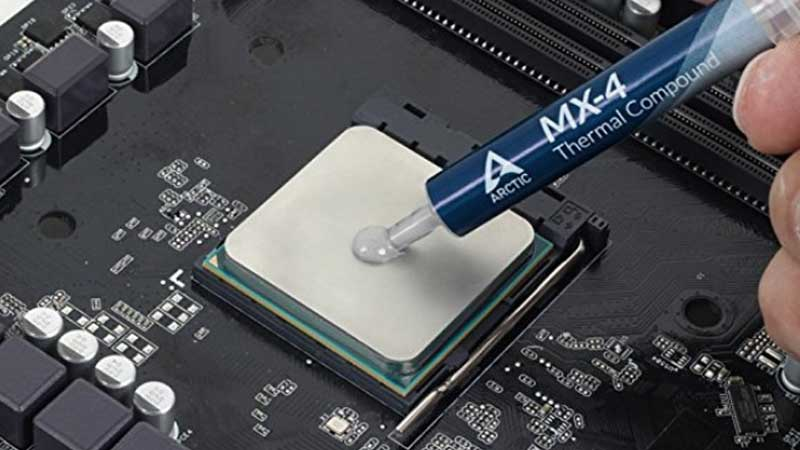
\includegraphics[width=0.25\textwidth]{thermal.jpg}
	\caption{Pasta térmica}
\end{figure}


\subsection{Zócalo de CPU (\textit{CPU Socket})}

Este elemento se encarga de conectar el microprocesador (CPU) con la placa base de forma que la CPU pueda cambiarse sin necesidad de soldaduras. Existen varios tipos de zócalo:
\begin{itemize}
	\item \textit{PGA-ZIF, \textbf{P}in \textbf{G}rid \textbf{A}rray - \textbf{Z}ero \textbf{I}nsertion \textbf{F}orce}. La placa tiene agujeros en los que entran los pines de la CPU. Se utiliza una palanca para fijar la CPU al zócalo.
	\item \textit{LGA, \textbf{L}and \textbf{G}rid \textbf{A}rray}. La CPU tiene contactos y la placa base una matriz de superficies conductoras, de forma que así los pines no pueden doblarse. La CPU se asegura mediante una placa de metal.
\end{itemize}

\begin{figure}[H]
	\centering
	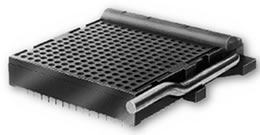
\includegraphics[width=0.25\textwidth]{pgazif.jpg}
	\caption{Socket \textit{PGA-ZIF}}
\end{figure}
\begin{figure}[H]
	\centering
	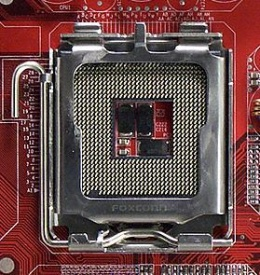
\includegraphics[width=0.25\textwidth]{lga.jpeg}
	\caption{Socket \textit{LGA}}
\end{figure}


\subsubsection{Historia de las CPU}
\begin{itemize}
	\item La litografía de las CPUs (tamaño de los transistores) ha ido descendiendo exponencialmente, lo que hace que se puedan incorporar más transistores.
	\item El número de transistores ha ido creciendo exponencialmente, lo que hace que crezca el rendimiento.
	\item Surge la Ley de Moore: cada dos años se duplica el número de transistores de un procesador.
	\item La frecuencia de reloj subía exponencialmente, al igual que el consumo.
	\item En 2005 se llegó a la barrera térmica (más calor haría que el chip se quemase). La frecuencia a la que se llegó fue de unos 4.2Ghz.
	\item La competitividad se centra actualmente en fabricar CPUs con más caché, más núcleos, controlador gráfico integrado, etc. (la lucha por la máxima frecuencia terminó).
\end{itemize}

\begin{figure}[H]
	\centering
	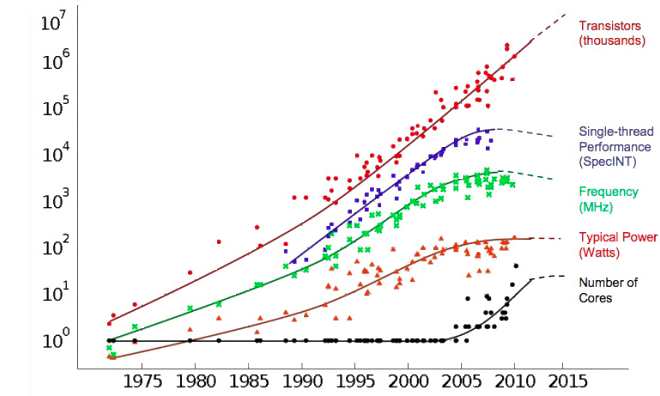
\includegraphics[width=0.5\textwidth]{cpuhistory.png}
	\caption{Evolución histórica de las CPU}
\end{figure}

Hoy día los principales fabricantes de CPU son IBM, Intel y AMD.

\subsubsection{Intel Xeon}

Son la división de procesadores Intel específica para servidores. Incorporan más soporte para multiprocesamiento, más tecnologías (como \textit{HyperThreading}, capaz de realizar la emulación de dos hebras mediante un único núcleo) y, en general, mayores prestaciones que las de un equipo sobremesa.\\

Una CPU para servidores es capaz de coexistir con otra CPU en la misma placa. Sin embargo, esto acarrea un problema: si una CPU quiere acceder a un banco de memoria de la otra, necesita pasar por la otra CPU de forma muy rápida. Para solucionar esto surgen los \textit{UPI Link}, conexiones muy rápidas entre las CPUs. Cuantos más \textit{UPI Links} tenga una CPU, mayor velocidad de acceso tendrá.

\begin{figure}[H]
	\centering
	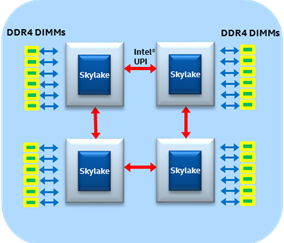
\includegraphics[width=0.5\textwidth]{upi.png}
	\caption{Esquema de funcionamiento de los \textit{UPI Links} (flechas rojas)}
\end{figure}

Estos procesadores suelen soportar memoria ECC (\textit{Error Correcting Code}). Estas memorias incorporan un chip más (8 bits de redundancia para detectar si hay un error y corregirlo).

\subsubsection{AMD (EPYC y Opteron)}

Son los procesadores de AMD dedicados para servidores. El primer Opteron (presentado en 2003) fue el primer procesador que utilizaba el conjunto de instrucciones AMD x86-64. Por ser AMD la primera marca en lanzar un procesador x86-64, hoy día las distribuciones de 64 bits se siguen llamando AMD64.\\

Actualmente hay tres grandes familias de CPUs AMD para servidores:
\begin{itemize}
	\item EPYC.
	\item Opteron X-Series (basada en APU, \textit{Accelerated Processing Unit}). Incorporan CPU y GPU en un mismo chip, además de E/S (son un SoC, \textit{System on a Chip}). Intel también incorpora una GPU en muchos de sus procesadores. Usan la arquitectura x86
	\item Opteron A-Series. Utilizan el repertorio ARM. Tienen un gran ratio prestaciones/consumo y son SoC con controladores PCI-e, Ethernet y SATA en el propio chip. Consumen menos de 30W.
\end{itemize}

\subsubsection{IBM Power (\textit{Performance Optimization With Enhanced RISC})}

IBM fabrica grandes máquinas con muchas E/S. Esto aporta gran fiabilidad y redundancia.\\

El procesador más destacado es el \textbf{IBM Power 9}. Sus características más importantes son que la memoria caché L3 es distribuida y que cada núcleo puede ejecutar hasta 8 hilos.

\subsection{Ranuras para la memoria DRAM (\textit{Dynamic Random Access Memory})}

Son los conectores donde se insertan los módulos de memoria principal, que tiene una velocidad inferior a la SRAM (caché) pero mayor densidad.\\

La DRAM tiene las siguientes características:
\begin{itemize}
	\item Se comunica con la CPU mediante un bus de 64 bits.
	\item RW: lectura y escritura.
	\item Volátil: al apagar la máquina se elimina su contenido.
	\item Necesita refresco: la información se desvanece si no se leen y reescriben los datos cada X tiempo. De esto se encarga un controlador dedicado.
	\item Tiene una mayor densidad, ya que cada celda es mucho más simple.
\end{itemize}
\begin{figure}[H]
	\centering
	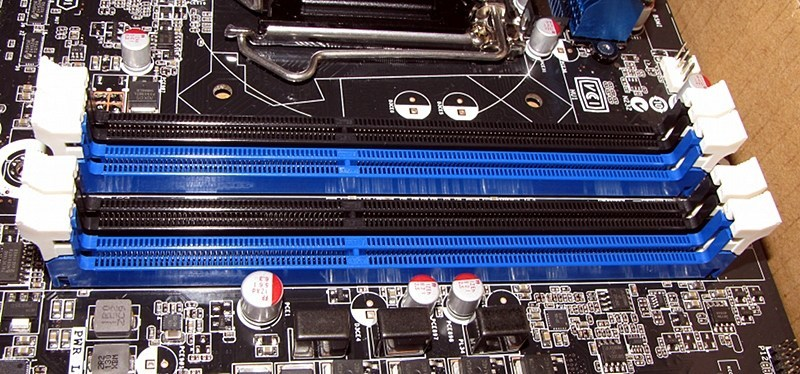
\includegraphics[width=0.5\textwidth]{ramslot.jpg}
	\caption{Slot para memoria RAM}
\end{figure}
\begin{figure}[H]
	\centering
	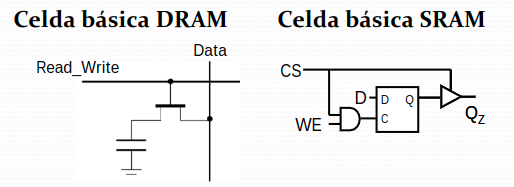
\includegraphics[width=0.5\textwidth]{ramcells.png}
	\caption{Celdas DRAM y SRAM}
\end{figure}

\subsubsection{Evolución histórica de la DRAM}
\begin{itemize}
	\item Se comienza con la \textbf{SDRAM}: Synchronous DRAM. Hay una señal de reloj para saber cuándo se podrá obtener el dato.
	\item Tras las memorias síncronas, la competitividad se centra en obtener más datos por cada ciclo de reloj (DDR: 2 datos, DDR2, 4 datos, ..., DDR4: 8 datos).
	\item Con el paso del tiempo el número de conectores de cada módulo ha ido aumentando.
	\item El voltaje ha ido descendiendo con los años (lo que acarrea un menor consumo).
	\item Desde DDR2 el bus de datos se ha estancado en 64 bits. Cada vez que la CPU pide un dato, se le mandan 64 bits. El bus se usa para lectura y escritura a la vez, por lo que no se pueden realizar las dos operaciones al mismo tiempo (\textit{half-duplex}).
	\item El ancho de banda (\textit{throughput}, productividad) ha ido aumentando con los años.
\end{itemize}

Los tipos de memorias RAM son los siguientes:

\begin{itemize}
	\item \textit{SIPP: \textbf{S}inge \textbf{I}n-line \textbf{P}in \textbf{P}ackage}.
	\item \textit{SIMM: \textbf{S}inge \textbf{I}n-line \textbf{M}emory \textbf{M}odule}.
	\item \textit{DIMM: \textbf{D}ual \textbf{I}n-line \textbf{M}emory \textbf{M}odule}.
\end{itemize}

\begin{figure}[H]
	\centering
	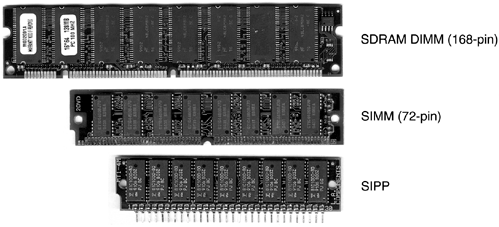
\includegraphics[width=0.7\textwidth]{ramtypes.png}
	\caption{Tipos de RAM}
\end{figure}

\subsubsection{Tipos de memoria DIMM}

\begin{itemize}
	\item DIMM o U-DIMM (\textit{Unbuffered DIMM}). No tienen registro (buffer). Son las que se utilizan en los PC.
	\item EU-DIMM: son U-DIMM con ECC.
	\item R-DIMM (\textit{Registered DIMM}). Hay un registro que almacena las señales de control, por lo que los módulos pueden tener mayor capacidad. Como consecuencia la latencia es mayor, ya que hay que acceder al registro antes que a la celda. Tienen ECC.
	\item LR-DIMM (\textit{Load Reduced DIMM}). El registro almacena tanto las señales de control como el dato a manejar. Por tanto, son las que admiten más memoria. Son también las más caras. Tienen ECC.
	\item SO-DIMM (\textit{Small Outline DIMM}). Son más pequeñas, ya que se utilizan en portátiles (tienen menos contactos).
\end{itemize}

\subsubsection{Canales y bancos de memoria DRAM}

Un banco de memoria es un grupo de módulos que comparten canal de memoria. No se puede acceder en paralelo a dos módulos bajo un mismo banco, pero sí a distintos bancos.\\

Los canales unen los bancos con la CPU.

\begin{figure}[H]
	\centering
	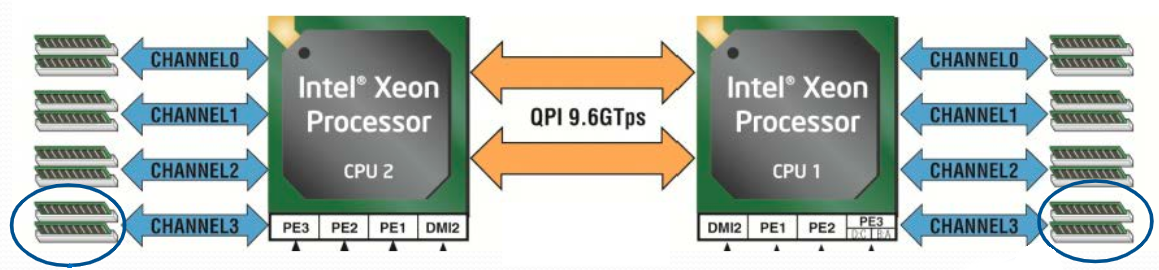
\includegraphics[width=0.7\textwidth]{rambanks.png}
	\caption{Canales (flechas) y banos (rodeados) de RAM}
\end{figure}

\subsubsection{Rangos de memoria RAM}

Los rangos son agrupaciones de memoria que suman una palabra completa (64 bits o 72 si la memoria tiene ECC). La notación utilizada es la siguiente:
\begin{itemize}
	\item 1Rx4: módulo de un rango con chips de 4 bits ($\frac{64}{4}= 16$ chips por rango).
	\item 2Rx8: módulo de dos rangos con chips de 8 bits ($\frac{64}{8}= 8$ chips por rango). Por ejemplo, un módulo con dos caras, cada una con un rango de 8 chips de 8 bits cada uno.
\end{itemize}

Algunas CPUs pueden no soportar un determinado número de rangos.

\begin{figure}[H]
	\centering
	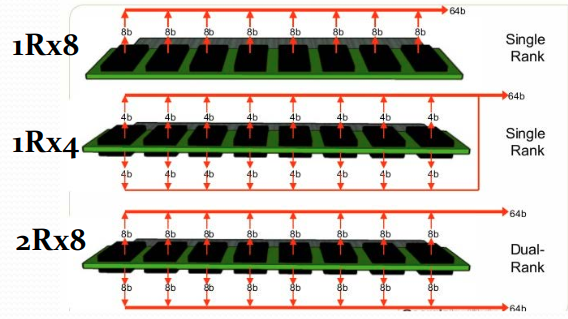
\includegraphics[width=0.7\textwidth]{ramranks.png}
	\caption{Notación de rangos de RAM}
\end{figure}

En las especificaciones de una memoria DRAM suelen aparecer los siguientes campos:
\begin{itemize}
	\item DDR4-\textbf{2166}. Es la frecuencia efectiva. El módulo puede realizar 2666 MegaTransferencias por segundo. Como cada transferencia es de 64 bits (8 bytes): $2166 MTps * 8 B= 21328Mbps \approx$ 21300.
	\item DDR4-PC4-\textbf{21300}. Viene del apartado anterior.
	\item CL19. Latencia de acceso de 19 ciclos de reloj. Hemos de tener cuidado, ya que la velocidad depende tanto de la latencia como de la frecuencia.
	\item \textit{x4 based}. Cada chip aporta 4 bits (por tanto, si la memoria tiene ECC, hay $\frac{72}{4}=18$ módulos en cada cara).
	\item \textit{Dual Ranked}. En la otra cara hay otros 18 módulos.
\end{itemize}

\subsection{Ranuras de expansión}

Sireven para extender la funcionalidad de la placa base mediante otras tarjetas PCB. Los principales slots son:
\begin{itemize}
	\item \textbf{ISA} (\textit{\textbf{I}ndustry \textbf{S}tandard \textbf{A}rchitecture}). Usaban un bus de 16 bits en half-dúplex (el mismo bus se usaba para lectura y escritura).
	\item \textbf{PCI} (\textit{\textbf{P}eripheral \textbf{C}omponent \textbf{I}nterconnect}). Fueron lanzadas por Intel. Sus principales características son:
		\begin{itemize}
			\item \textit{Plug\&Play}: la tarjeta se conecta a la máquina y ya se puede usar. No se necesita especificar la interrupción con la que la máquina puede comunicarse con la tarjeta (en ISA sí).
			\item Se usa un bus paralelo (half-dúplex) de 32 ó 64 bits. La señal de reloj es igual para los 32 ó 64 bits.
			\item Existe una versión específica para servidores (PCI-X) que lograba un ancho de banda de prácticamente el doble.
		\end{itemize}
		\item \textbf{AGP} (\textit{\textbf{A}ccelerated \textbf{G}raphics \textbf{P}ort}). Desarrolladas por Intel. Es una conexión específica para GPUs, por lo que se eliminan características de PCI que utilizaban el resto de tarjetas.
		\item \textbf{PCIe} (\textit{PCI Express}). Es loa interfaz utilizada actualmente.
		\begin{itemize}
			\item Se usa una conexión en serie punto a punto (las líneas no son compartidas) por medio de \textit{LANES}.
			\item Cada \textit{LANE} está compuesta por 4 cables: dos para leer y 2 para escribir (full-dúplex) .
			\item Cada \textit{LANE} tiene su propia señal de reloj (incrustada en los datos que transfiere).
			\item \textit{Hot plug}, es decir, podemos conectar la tarjeta a la máquina sin apagarla, ya que el número de \textit{LANES} se negocia automáticamente.
			\item Se virtualiza la E/S (el hipervisor de una máquina virtual no tiene que gestionar el acceso al recurso, sino que la tarjeta reserva una parte para la MV	item).
			\item La escalabilidad es muy sencilla, sólo hay que incrementar el número de \textit{LANES}.
			\item Se añade redundancia, por lo que las codificaciones más comunes son 8b/10b (el dato ocupa 8 bits pero se añaden 2 más de redundancia) y 128b/130b.
			\item Las versiones de PCIe y sus respectivas velocidades (en cada línea y sentido) son las siguientes:
			\begin{itemize}
				\item PCIe 1.1: 2.5GT/s (250MB/s). En la codificación 8b/10b dividimos las gigatransferencias entre 10 para hallar la velocidad en MB/s.
				\item PCIe 2.0: 5GT/s (500/s)
				\item PCIe 3.0: 8GT/s (en torno a 1GB/s). Aquí se comenzó a usar la codificación 128b/130b, por lo que dividimos entre 8.
				\item PCIe 4.0: 16GT/s (en torno a 2GB/s)
			\end{itemize}
			\item El número de \textit{LANES} habitual es x1,x2,x4,x8 o x16 (tarjetas gráficas).
			\item Las principales ventajas de utilizar un protocolo de serie con respecto a uno paralelo son el aumento de frecuencia de reloj (lo que evita el \textit{timing skew}, fenómeno por el que una señal de reloj llega a distintos componentes en tiempos distintos debido a que la longitud del cable es distinta) y una mayor escalabilidad.
		\end{itemize}
\end{itemize}

\begin{figure}[H]
	\centering
	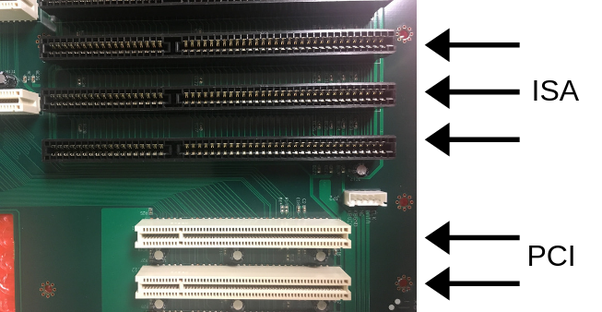
\includegraphics[width=0.75\textwidth]{isapci.png}
	\caption{Slots ISA y PCI}
\end{figure}

\begin{figure}[H]
	\centering
	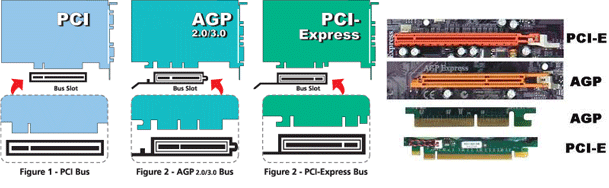
\includegraphics[width=\textwidth]{pcieagp.png}
	\caption{Slots PCI, AGP y PCI Express}
\end{figure}

\begin{figure}[H]
	\centering
	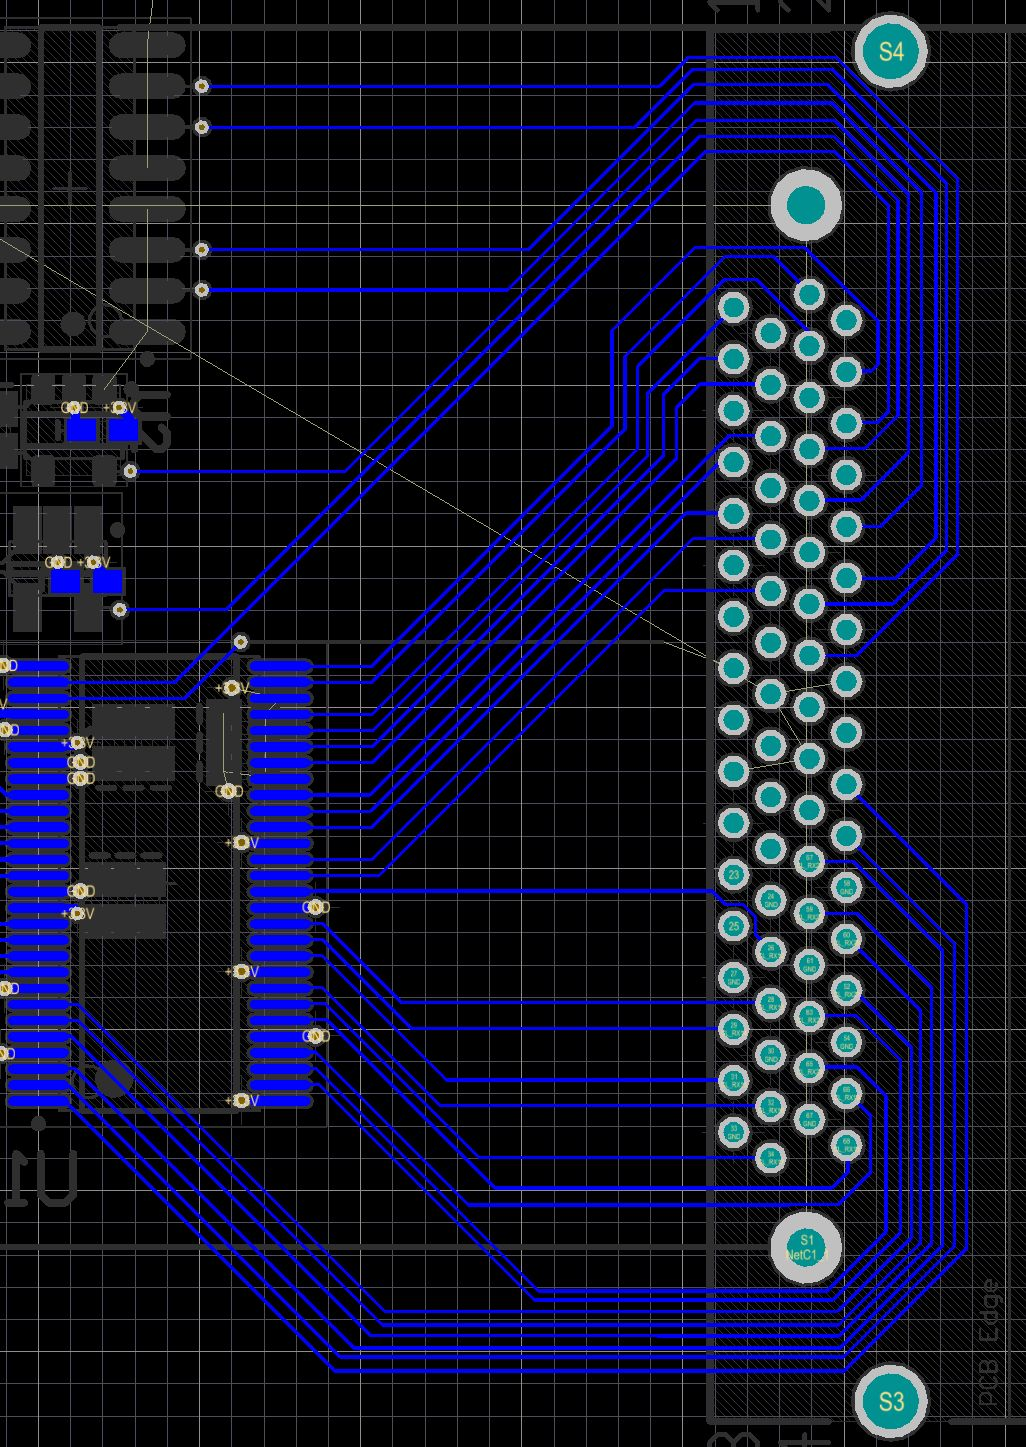
\includegraphics[angle=90,width=0.5\textwidth]{timskew.jpg}
	\caption{Las líneas no tienen la misma longitud, lo que provoca el \textit{timing skew}}
\end{figure}

\subsection{Almacenamiento permanente (no volátil)}

Estos dispositivos sirven para almacenar información sin que se pierda al apagar la máquina. Se dividen en :
\begin{itemize}
	\item Según su tipo:
	\begin{itemize}
		\item Magnéticos (disquetes, HDD, cintas).
		\item Ópticos (CD, DVD, Blu-Ray).
		\item Memoria Flash (SSD).
	\end{itemize}
	\item Según su factor de forma (en pulgadas): 3.5, 2.5 y 1.8.
	\item Según su conexión a la placa base: ATA (IDE), SATA, M.2, SCSI, SAS, etc,
\end{itemize}

\subsubsection{Discos duros (HDD)}
\begin{itemize}
	\item Son discos recubiertos de un material magnético. La lectura y escritura se realiza mediante un cabezal magnético móvil.
	\item Los datos se distribuyen en pistas.
	\item Las pistas se dividen en sectores, que se agrupan en clústers lógicos.
	\item Si incrementamos las revoluciones por minuto (normalmente 5400, 7200 o 10000), aumentamos la productividad y el ancho de banda.
	\item La latencia es variable: depende de dónde se encuentre el cabezal y dónde el dato.
	\item Se suele añadir un módulo de caché para acelerar la lectura.
\end{itemize}

\begin{figure}[H]
	\centering
	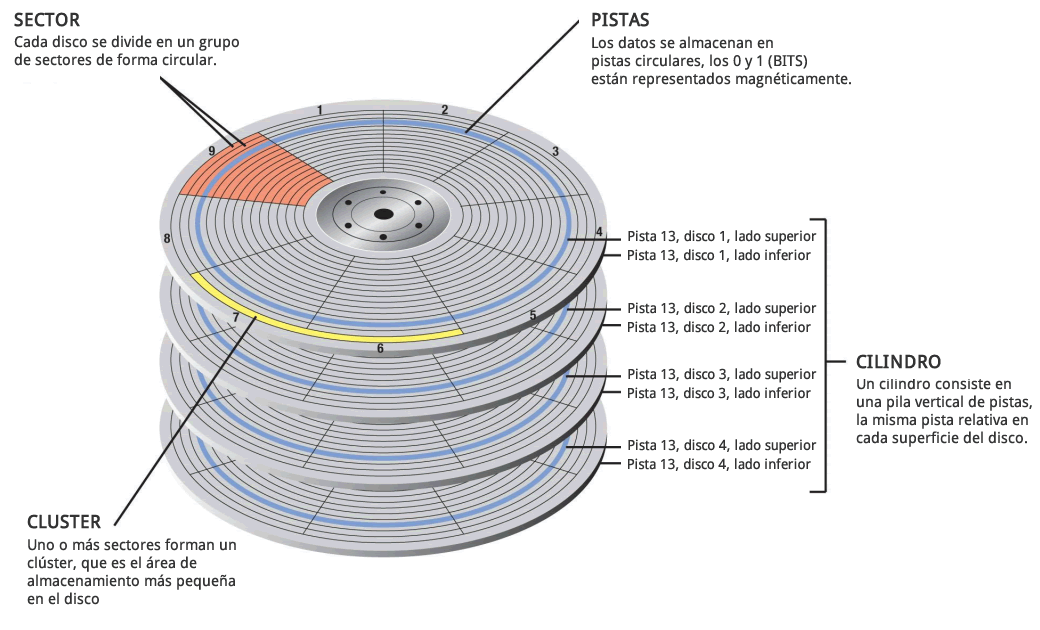
\includegraphics[width=0.75\textwidth]{hddparts.png}
	\caption{Pistas, sectores, clústers y cilindros en un HDD}
\end{figure}

\subsubsection{Unidades de estado sólido (SSD)}
\begin{itemize}
	\item Están basadas en MOSFETs de puerta flotante.
	\item Se obtiene la misma latencia accediendo a cualquier dato.
	\item La densidad de chips es más baja, por lo que la capacidad también.
	\item Las celdas más comunes son MLC (\textit{\textbf{M}ulti \textbf{L}evel \textbf{C}ell}) que admiten más de dos estados. Por ejemplo: descargado, poco cargado, muy cargado y completamente cargado.
	\item Un controlador se encarga de distribuir la información entre las celdas para equilibrar el número de escrituras (\textit{wear leveling}) y así prolongar la vida útil de la unidad.
\end{itemize}

\begin{figure}[H]
	\centering
	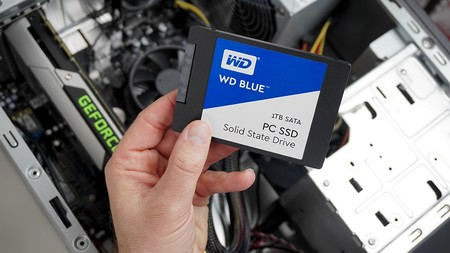
\includegraphics[width=0.5\textwidth]{ssd.jpg}
	\caption{SSD}
\end{figure}

\begin{figure}[H]
	\centering
	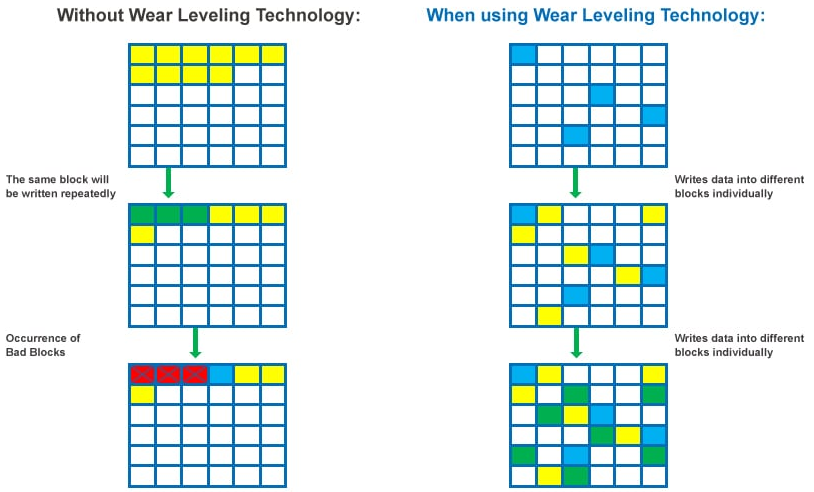
\includegraphics[width=\textwidth]{wearleveling.png}
	\caption{La importancia de \textit{wear leveling}}
\end{figure}

\subsubsection{RAID}
Consiste en combinar distintas unidades de almacenamiento para generar unidades lógicas con mayor tolerancia a fallos, fiabilidad y ancho de banda. Puede estar creado por software o por hardware (una tarjeta específica).

\subsubsection{Unidades ópticas}
Almacenan información de forma permanente a partir de surcos en un disco que se pueden leer mediante un haz de luz láser. Su principal problema es que no tienen un gran ancho de banda. Los más comunes son el CD, DVD y Blu-Ray.

\begin{figure}[H]
	\centering
	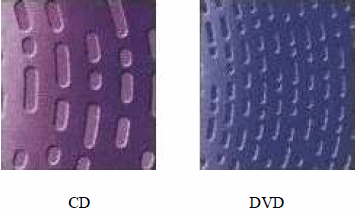
\includegraphics[width=0.5\textwidth]{surcos.png}
	\caption{Surcos en un CD y un DVD}
\end{figure}

\subsubsection{Unidades de cinta}

\begin{itemize}
	\item Almacenan información a través de una cinta recubierta de material magnético que se enrolla en carretes.
	\item La latencia suele ser alta ya que hay que rebobinar la cinta para que el cabezal lea lo adecuado.
	\item Es el medio con mayor densidad de bits (decenas de TB por cinta).
	\item Es el medio de almacenamiento masivo más barato.
	\item Se utiliza normalmente como backup.
\end{itemize}

\subsubsection{Interfaz P-ATA (\textit{\textbf{P}arallel \textbf{A}dvanced \textbf{T}echnology \textbf{A}ttachment})}

\begin{itemize}
	\item Utiliza el conector IDE (\textit{\textbf{I}ntegrated \textbf{D}evice \textbf{E}lectronics}).
	\item Emplea una faja de 40 pines con un bus paralelo (half-dúplex) de 16 bits que permite conectar dos dispositivos (maestro y esclavo).
	\item Transfiere un máximo de 133Mbps.
	\item La longitud máxima de la faja es de 45cm.
\end{itemize}


\begin{figure}[H]
	\centering
	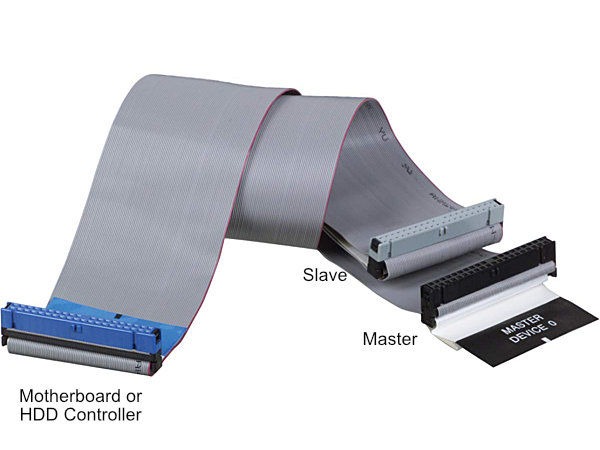
\includegraphics[width=0.5\textwidth]{patacable.jpg}
	\caption{Faja PATA}
\end{figure}

\begin{figure}[H]
	\centering
	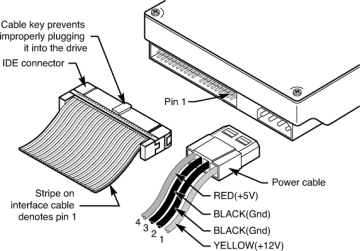
\includegraphics[width=0.5\textwidth]{pataconnection.jpg}
	\caption{Conexión de un dispositivo PATA}
\end{figure}

\subsubsection{S-ATA (\textit{\textbf{S}erial \textbf{ATA}})}
\begin{itemize}
	\item Emplea un bus serie punto a punto full-dúplex (2 cables para leer y 2 para escribir).
	\item Permite una unidad por conector.
	\item La longitud máxima del cable es de 1m.
	\item Emplea AHCI (\textit{\textbf{A}dvanced \textbf{H}ost \textbf{C}ontroller \textbf{I}nterface}), un estándar que define dos elementos:
	\begin{itemize}
		\item Hot plug: podemos conectar el disco en caliente.
		\item NCQ (\textit{\textbf{N}ative \textbf{C}ommand \textbf{Q}uery}). Aumenta el rendimiento de los discos rotacionales implementando una cola de prioridad en la que se leen los datos no según el orden de llegada de la petición, sino según su distancia a la posición actual de la aguja.
	\end{itemize}
	\item Las distintas versiones de SATA son: SATA1 (1500Mhz, 150MB/s), SATA2 (3000Mhz, 300MB/s) y SATA3 (6000Mhz, 600MB/s). Dividimos los Mhz entre 10 para obtener los MB/s.
\end{itemize}

\begin{figure}[H]
	\centering
	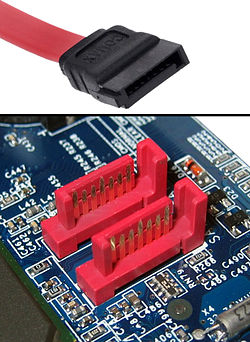
\includegraphics[width=0.3\textwidth]{sata.jpg}
	\caption{Cable y conector SATA}
\end{figure}

\begin{figure}[H]
	\centering
	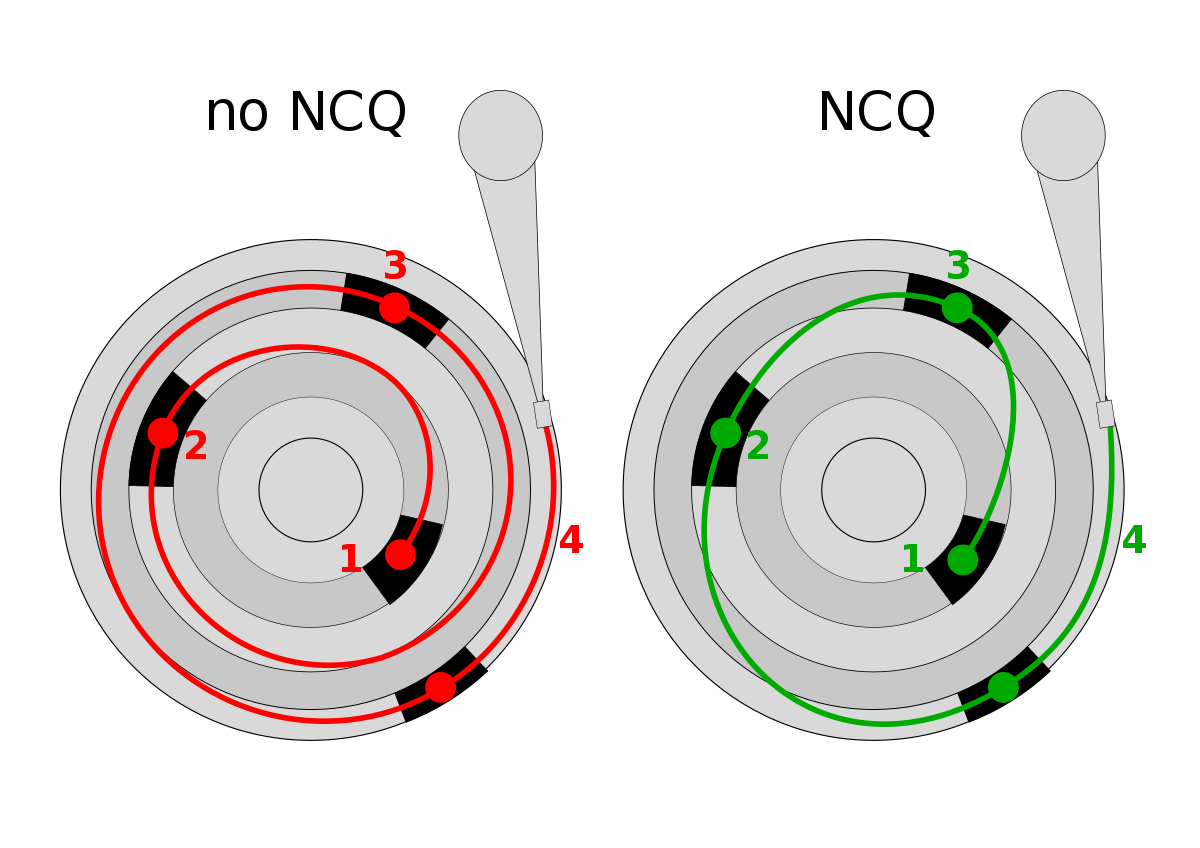
\includegraphics[width=0.5\textwidth]{ncq.png}
	\caption{Funcionamiento de NCQ}
\end{figure}

\subsubsection{SCSI y SAS}

\begin{itemize}
	\item SCSI (\textit{\textbf{S}mall \textbf{C}omputer \textbf{S}ystem \textbf{I}nterface})
	\begin{itemize}
		\item Utiliza un bus paralelo de 16 bits half-dúplex.
		\item Es más veloz que ATA.
		\item Soporta Hot Plug.
		\item Permite conectar varias unidades en cadena (\textit{daisy-chain}).
	\end{itemize}
	\item Ultra-SCSI: permite hasta 320MB/s y 12m de cable. Emplea half-dúplex también.
	\item SAS (\textit{\textbf{S}erial \textbf{A}ttached \textbf{SCSI}}). Es la versión serie de SCSI.
	\begin{itemize}
		\item Permite velocidades de hasta 12Gbps.
		\item Soporta full-dúplex.
		\item Es compatible con SATA pero usa mayores voltajes (por ello el conector de alimentación se une al de datos).
		\item Permite hasta 10 metros de cable.
		\item Se pueden conectar varias unidades al mismo puerto mediante conectores mini-SAS (4 unidades por puerto mediante un cable \textit{splitter}).
		\item También se puede emplear un expansor SAS para conectar más unidades a la placa base.
	\end{itemize}
\end{itemize}

\begin{figure}[H]
	\centering
	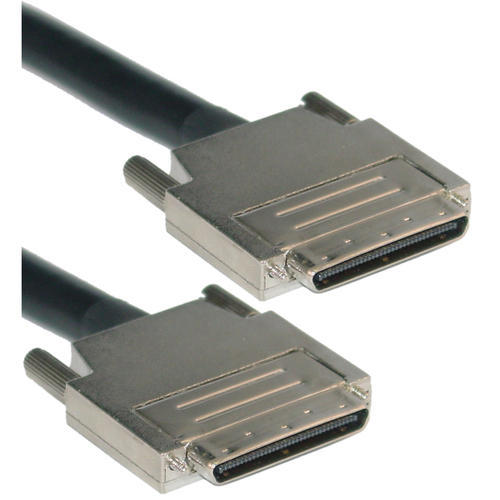
\includegraphics[width=0.3\textwidth]{scsicable.jpg}
	\caption{Cable SCSI}
\end{figure}

\begin{figure}[H]
	\centering
	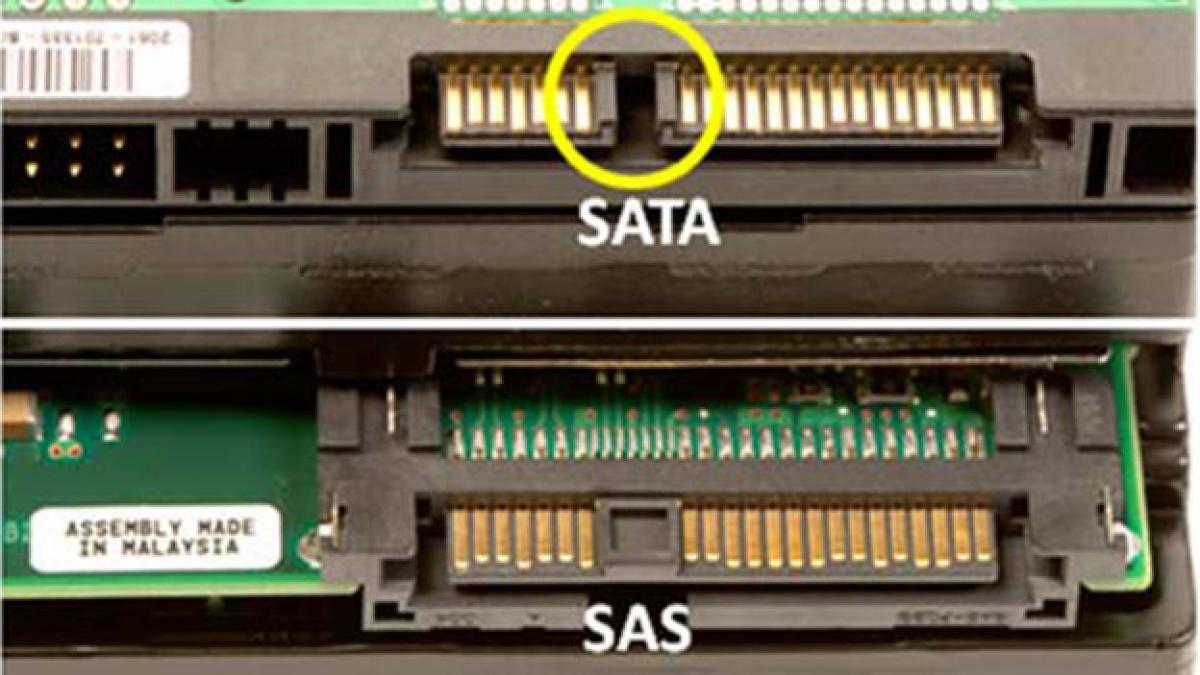
\includegraphics[width=0.5\textwidth]{sasconnector.jpg}
	\caption{Conectores SATA y SAS}
\end{figure}

\begin{figure}[H]
	\centering
	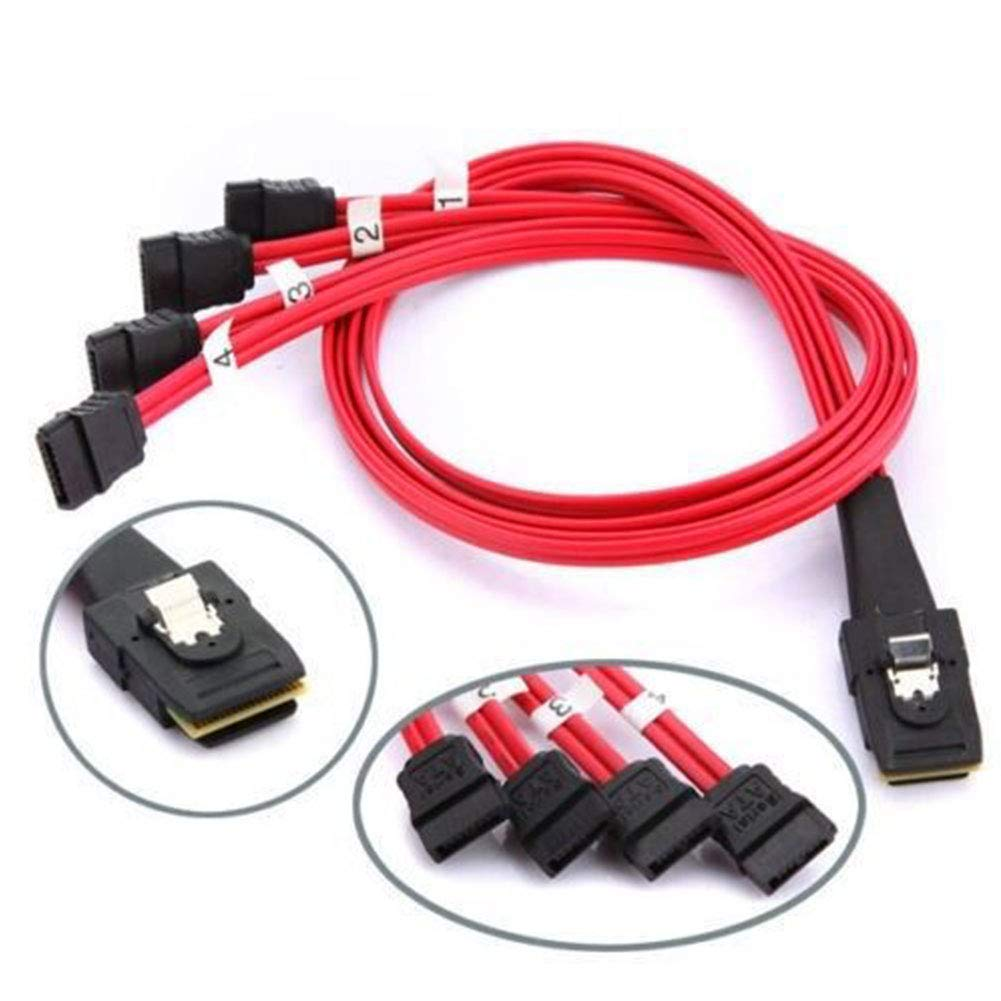
\includegraphics[width=0.35\textwidth]{sassplitter.jpg}
	\caption{Cable \textit{splitter} SAS}
\end{figure}

\begin{figure}[H]
	\centering
	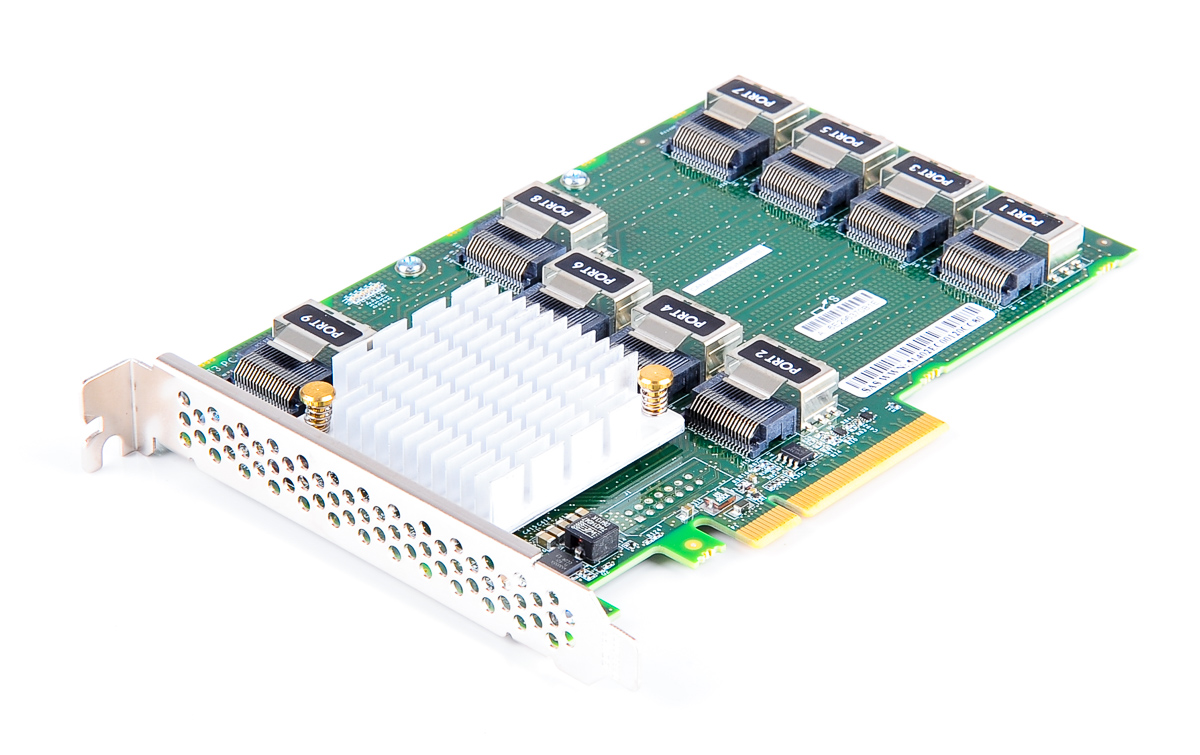
\includegraphics[width=0.35\textwidth]{sasexpander.jpg}
	\caption{Expansor SAS}
\end{figure}

\subsubsection{NVMe (\textbf{N}on \textbf{V}olatile \textbf{M}emory \textbf{E}xpress)}
Se trata de un protocolo para conectar unidades SSD mediante PCIe (normalmente x4). Su mayor ventaja es la gran escalabilidad que proporciona. Se implementan en los siguientes conectores:
\begin{itemize}
	\item PCIe x4, 4GB/s.
	\item M.2. Es el mini-sata de segunda generación. Usa internamente PCIe x4 (4GB/s).
	\item U.2. Fue lanzado por Intel. Utiliza también PCIe x4 de forma interna (4GB/s).
	\item SATA3.2. Combina PCIe y SATA, llegando a 2GB/s.
\end{itemize}

\begin{figure}[H]
	\centering
	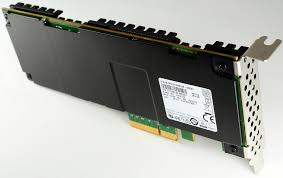
\includegraphics[width=0.35\textwidth]{pcienvme.jpeg}
	\caption{NVMe PCIe}
\end{figure}

\begin{figure}[H]
	\centering
	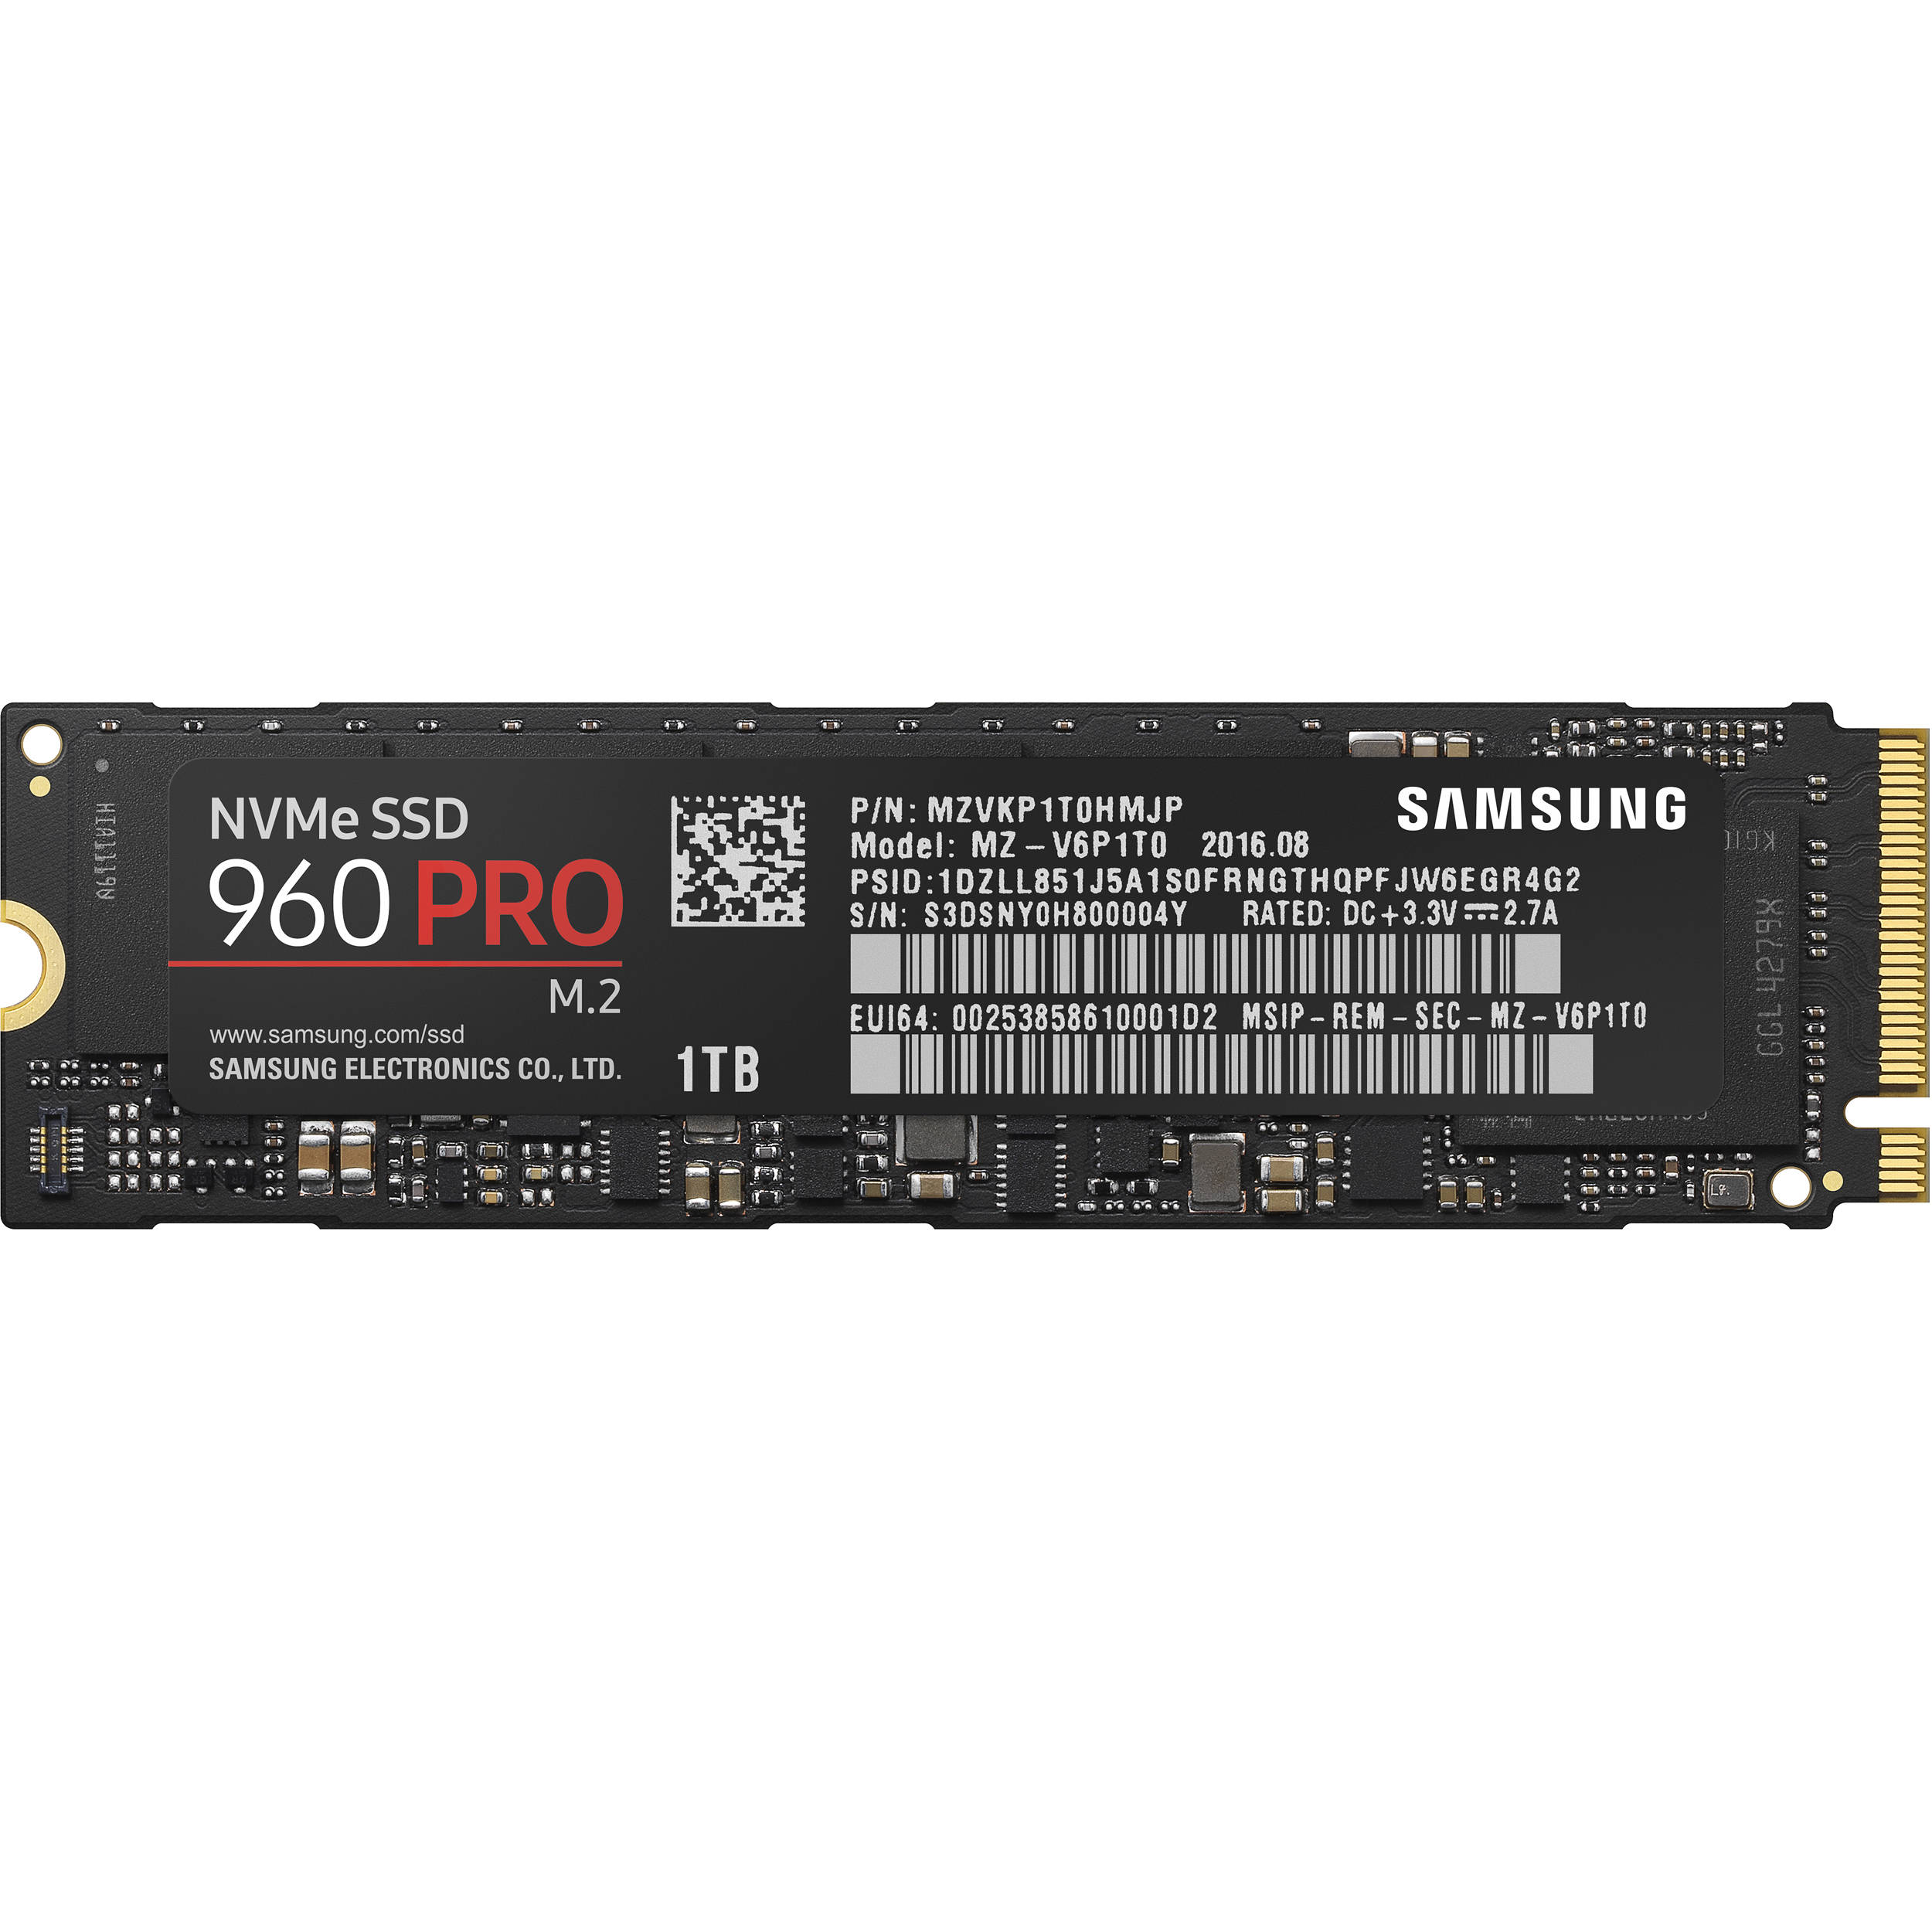
\includegraphics[width=0.35\textwidth]{m2.jpg}
	\caption{NVMe M.2}
\end{figure}

\begin{figure}[H]
	\centering
	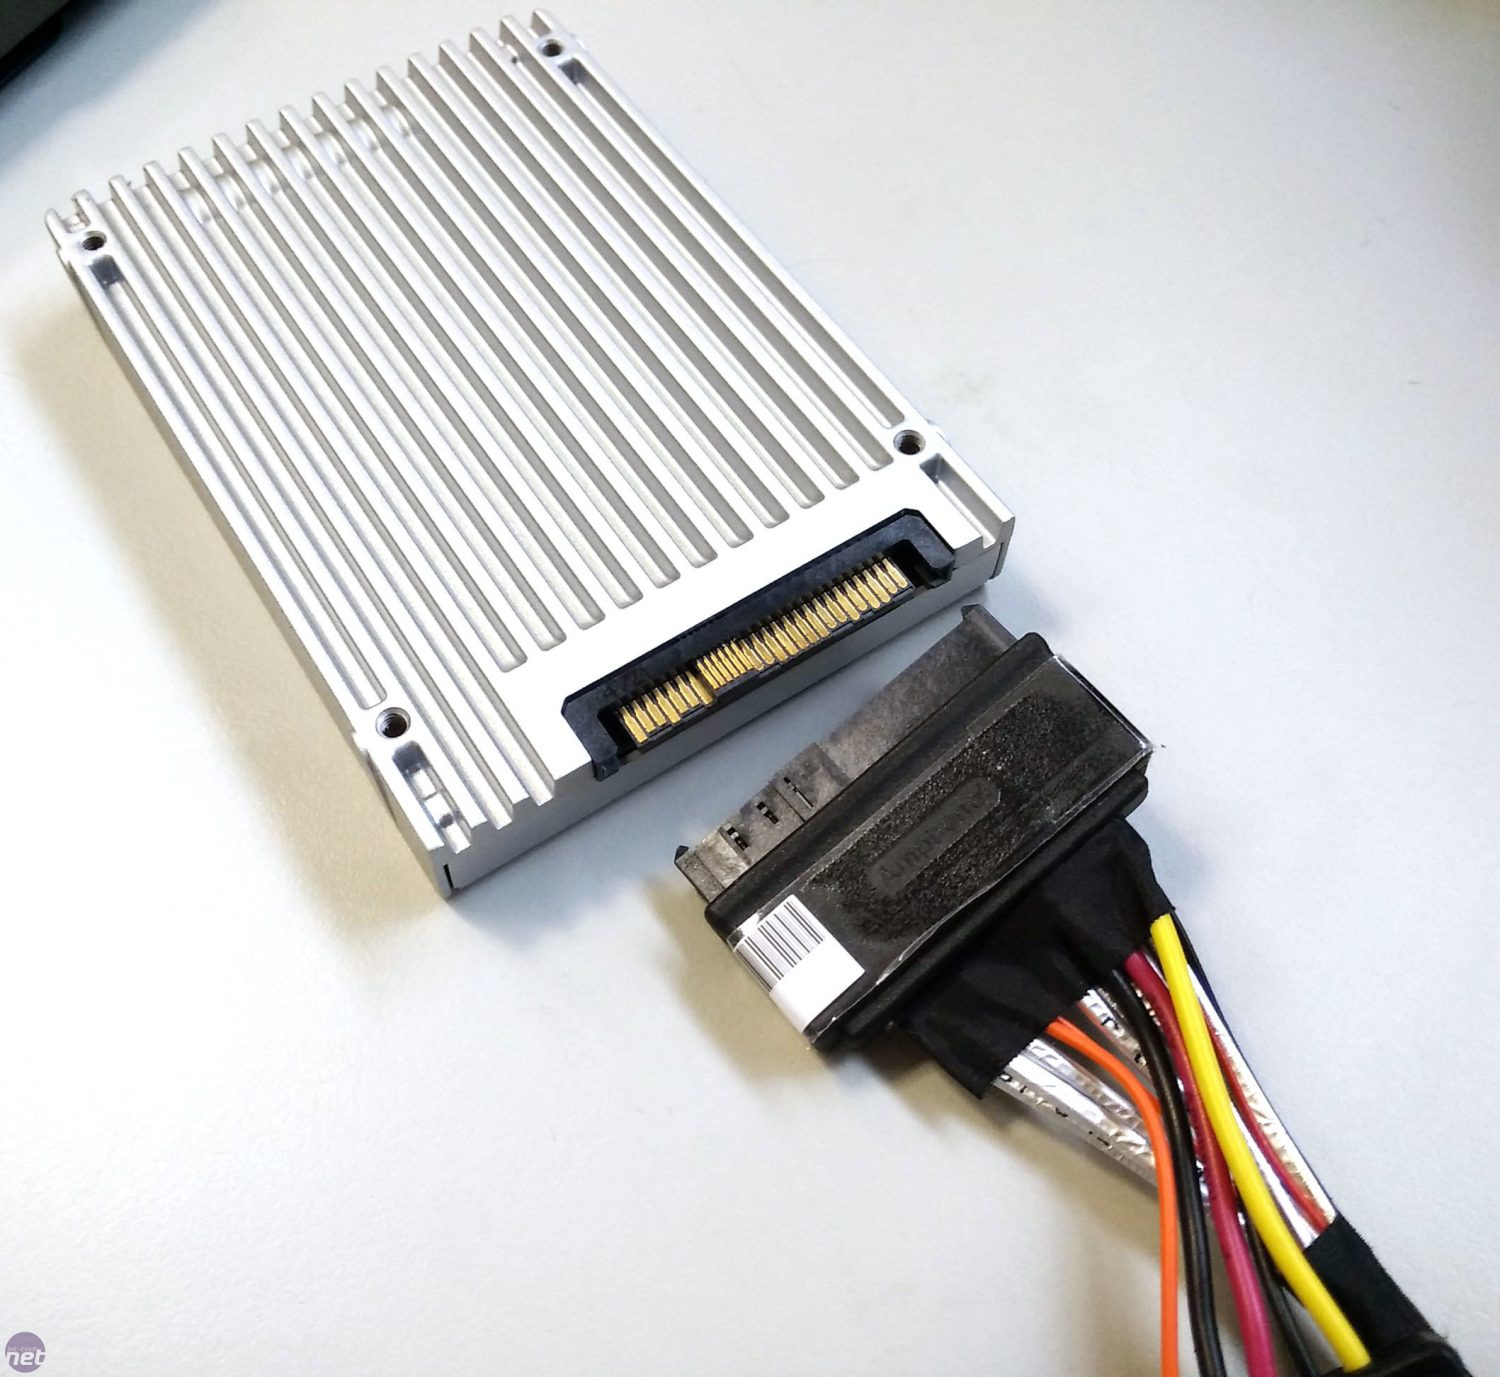
\includegraphics[width=0.35\textwidth]{u2.jpg}
	\caption{NVMe U.2}
\end{figure}

\begin{figure}[H]
	\centering
	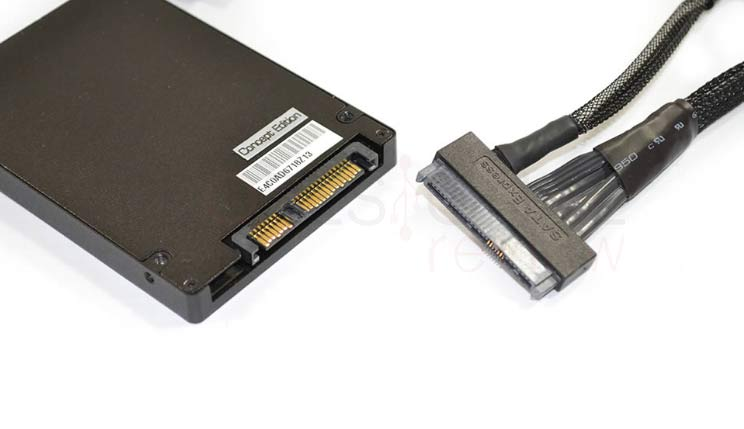
\includegraphics[width=0.35\textwidth]{satae.jpg}
	\caption{NVMe SATA Express}
\end{figure}

\subsubsection{Otras interfaces de almacenamiento}

\begin{itemize}
	\item \textbf{Fibra óptica}. Es una tecnología de red en serie constituida por dos fibras unidireccionales que transmiten en idrecciones opuestas. Permite conexión punto a punto, en anillo o redes conmutadas (muy escalable). Puede transmitir hasta distancias de kilómetros. Son utilizadas por el 90\% de las SAN.
	\item \textit{\textbf{Infiniband}}. Ofrece una comunicación en serie punto a punto de muy baja latencia entre procesadores y periféricos de alta velocidad. Se usa en redes conmutadas.
\end{itemize}

\begin{figure}[H]
	\centering
	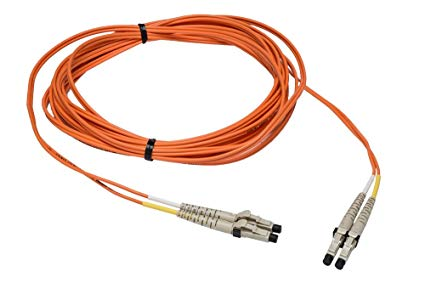
\includegraphics[width=0.35\textwidth]{fccable.jpg}
	\caption{Cable de fibra óptica}
\end{figure}

\begin{figure}[H]
	\centering
	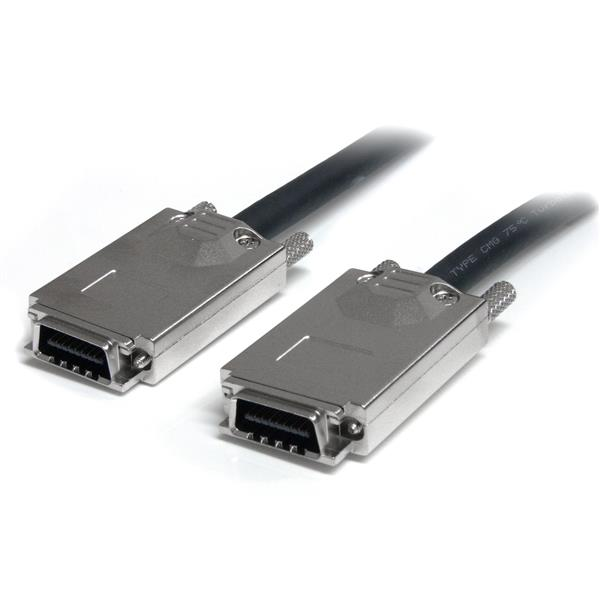
\includegraphics[width=0.35\textwidth]{infiniband.jpeg}
	\caption{Cable \textit{infiniband}}
\end{figure}

\subsection{Conectores del panel trasero}

Una placa base para servidor tiene en su panel trasero, básicamente:

\begin{itemize}
	\item Una salida de vídeo básica (normalmente VGA).
	\item Uno o varios conectores de red.
	\item Un conector de serie.
	\item USB.
\end{itemize}

Si la placa que estamos analizando tiene salidas de vídeo o audio de altas prestaciones, lo más seguro es que se trate de una placa para PC.

\begin{figure}[H]
	\centering
	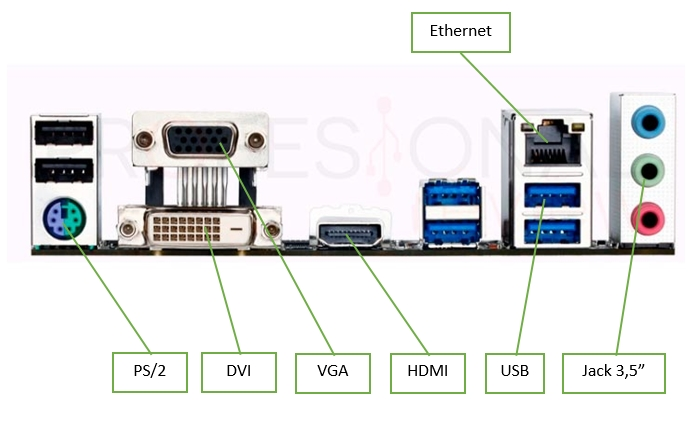
\includegraphics[width=0.8\textwidth]{pcmobo.jpg}
	\caption{Conectores de placa para PC}
\end{figure}

\begin{figure}[H]
	\centering
	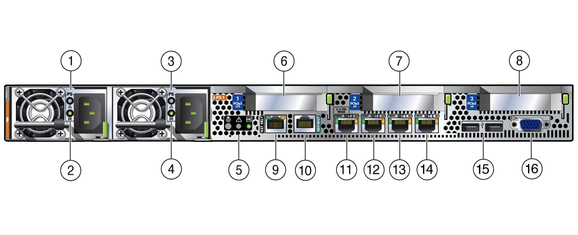
\includegraphics[width=0.8\textwidth]{serverconnectors.jpg}
	\caption{Conectores de placa para servidor}
\end{figure}

\subsection{RJ-45}

\begin{itemize}
	\item Sirve para conectar redes de área local a largas distancias (100m con par trenzado y varios km con fibra óptica).
	\item Los estándares son retrocompatibles y admiten full-dúplex.
	\item Muchos estándares de comunicación se pueden realizar a través de Ethernet:
	\begin{itemize}
		\item iSCSI (\textit{\textbf{I}nternet \textbf{SCSI}}): permite usar SCSI sobre redes TCP/IP.
		\item FCoE (\textit{\textbf{F}ibre \textbf{C}hannel \textbf{o}ver \textbf{Ethernet}}): permite usar tramas Fibre Channel sobre TCP/IP.
	\end{itemize}
\end{itemize}

\begin{figure}[H]
	\centering
	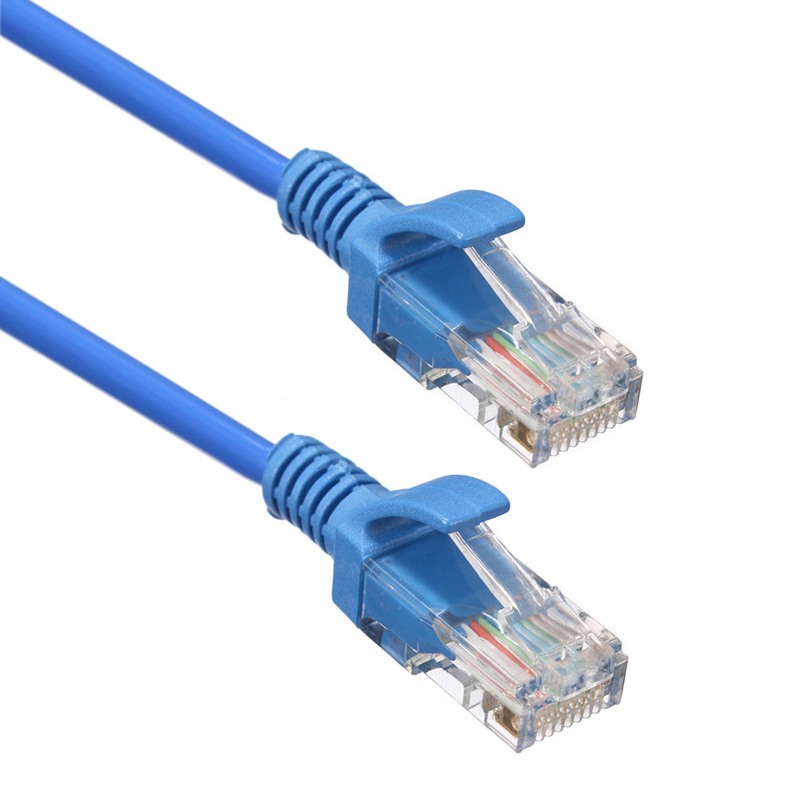
\includegraphics[width=0.3\textwidth]{rj45.jpg}
	\caption{Cable RJ-45}
\end{figure}

\subsection{Universal Serial Bus (USB)}

Actualmente se comercializan dos versiones:
\begin{itemize}
	\item USB 2.0
	\begin{itemize}
		\item Es un puerto de serie de 4 pines (2 de datos, 1 de masa y 1 de alimentación).
		\item Su velocidad máxima es de 480Mb/s.
		\item Soporta hot plug y opera mediante half-dúplex.
	\end{itemize}
	\item USB 3.0
	\begin{itemize}
		\item Se compone de 9 pines: 4 del USB 2.0 (es retrocompatible) y 5 para aportar más velocidad.
		\item Su velocidad máxima es de 4.8Gb/s.
		\item Su sucesor, USB 3.1, soporta hasta 10Gb/s.
	\end{itemize}
\end{itemize}

\begin{figure}[H]
	\centering
	\includegraphics[width=0.3\textwidth]{usb.png}
	\caption{Conectores USB 2.0 y 3.0}
\end{figure}

\subsection{Thunderbolt}

\begin{itemize}
	\item Es un estándar lanzado por Intel.
	\item Combina PCIe y DisplayPort (almacenamiento externo de altas prestaciones y monitor de alta resolución.
	\item Se alcanzan anchos de banda de hasta 40Gb/s en cada dirección y por cada canal.
	\item Utiliza el mismo conector que USB C.
\end{itemize}


\begin{figure}[H]
	\centering
	\includegraphics[width=0.3\textwidth]{thunderbolt.png}
	\caption{Cable Thunderbolt}
\end{figure}

\subsection{Otros conectores internos}

\subsubsection{System panel}

Sirve para conectar los botones de power y reset, luces de encendido y HDD, zumbador, etc. del chasis a la placa base.

\begin{figure}[H]
	\centering
	\includegraphics[width=0.5\textwidth]{syspanel.jpg}
	\caption{Conector del panel del sistema}
\end{figure}

\subsubsection{Puerto de serie}

Sirve para añadir un puerto de serie a la parte trasera de la máquina.


\begin{figure}[H]
	\centering
	\includegraphics[width=0.5\textwidth]{serial.jpg}
	\caption{Conector del puerto de serie}
\end{figure}

\subsubsection{USB interno}

Añade más puertos USB a la máquina. Pueden ser 2.0 o 3.0.

\begin{figure}[H]
	\centering
	\includegraphics[width=0.5\textwidth]{mobousb.jpg}
	\caption{Cable USB 3.0 y conectores USB (2.0 el blanco y 3.0 el azul)}
\end{figure}

\subsubsection{Chassis Intrusion Detector}

Envía una señal cuando se abre la tapa del chasis. Esta señal puede redirigirse a un administrador del sistema. Funciona con el voltaje 5V de standby.

\begin{figure}[H]
	\centering
	\includegraphics[width=0.5\textwidth]{chassisintrusion.jpg}
	\caption{Interruptor para detectar la intrusión en el chasis}
\end{figure}

\subsubsection{IEEE 1394a (Firewire)}

Sirve para conectar dispositivos en serie a gran velocidad. Fue sustituido por USB.

\begin{figure}[H]
	\centering
	\includegraphics[width=0.5\textwidth]{firewire.png}
	\caption{Conector Firewire}
\end{figure}

\subsubsection{CD IN audio}

Servía para el conector de audio de las lectoras de CD PATA. Fue sustituido por conectores de audio en el propio chasis.

\begin{figure}[H]
	\centering
	\includegraphics[width=0.5\textwidth]{cdin.jpg}
	\caption{Conector CD IN}
\end{figure}

\subsection{ROM/Flash BIOS (\textit{\textbf{B}asic \textbf{I}nput \textbf{O}utput \textbf{S}ystem})}

\begin{itemize}
	\item Almacena el código de arranque del computador, que se encarga de identificar los dispositivos instalador, instalar controladores básicos para poder acceder a ellos, realizar el POST (\textit{\textbf{P}ower \textbf{O}n \textbf{S}elf \textbf{T}est}) del sistema e iniciar el SO.
	\item Los parámetros de configuración se almacenan en una memoria RAM alimentada por una pila (que también se usa para el reloj de tiempo real). Algunos de estos parámetros se configuran mediante \textit{jumpers} (conectan dos o más pines) en la placa base, pero la mayoría se gestionan desde el firmware de la BIOS.
\end{itemize}

\begin{figure}[H]
	\centering
	\includegraphics[width=0.5\textwidth]{biosbattery.jpg}
	\caption{Chip BIOS y pila}
\end{figure}

\begin{figure}[H]
	\centering
	\includegraphics[width=0.5\textwidth]{bios.png}
	\caption{Firmware de la BIOS}
\end{figure}

\begin{figure}[H]
	\centering
	\includegraphics[width=0.5\textwidth]{jumper.jpg}
	\caption{\textit{Jumper} para borrar la configuración del firmware de la BIOS}
\end{figure}


%%%%%%%%%%%%%%%%%%%%%%%%%%%%%%%%%%%%%%%%%%%%%%%%%%%%%%%%%%%%%%%%%%%%%%%%%%%%%%%%%%%%%%%%%%%%%%%%%%%%%
\section{Ejercicios resueltos}
\subsection{Tema 1}
\begin{enumerate}
  \item[1.3] \label{1.13} Un  computador  tarda  100  segundos  en  ejecutar  un  programa  de  simulación  de  una  red  de  interconexión  para  multicomputadores.  El  programa  dedica  el 30\% en hacer operaciones de aritmética entera, el 60\% en hacer operaciones de aritmética  en  coma  flotante,  mientras  que  el  resto  se  emplea  en  operaciones  de  entrada/salida.  Calcule  la  ganancia  en  velocidad  y  el  tiempo  de  ejecución  si  las  operaciones  aritméticas  enteras  y  reales  se  mejoran de  manera  simultánea  2  y  3  veces, respectivamente.
	\begin{solution}
		\begin{figure}[H]
			\centering
			\begin{tikzpicture}[arrow/.style = {thick,-stealth}]
				\tikzset{set/.style={draw,rectangle,inner sep=0pt,align=center}}

				\node[fit={(0,0) (1,2.2)}, inner sep=0pt, draw=black, thick, fill=blue!20, text centered] (es) {\footnotesize E/S (\tiny $0.1*t_O=10s$)};
				\node[fit={(1,0) (7,2.2)}, inner sep=0pt, draw=black, thick, fill=green!20, text centered] (float) {Coma flotante (\footnotesize $0.6*t_O=60s$)};
				\node[fit={(7,0) (10,2.2)}, inner sep=0pt, draw=black, thick, fill=blue!20, text centered] (int) {Enteros (\footnotesize $0.3*t_O=30s$)};

				\node[fit={(0,-5) (1,-2)}, inner sep=0pt, draw=black, thick, fill=blue!20, text centered] (esm) {\footnotesize E/S (\tiny $0.1*t_O=10s$)};

				\node[fit={(1,-5) (3,-2)}, inner sep=0pt, draw=black, thick, fill=green!20, text centered] (floatm) {Coma flotante (\footnotesize $\frac{0.6*t_O}{3}=0.2*t_O=20s$)};

				\node[fit={(3,-5) (4.5,-2)}, inner sep=0pt, draw=black, thick, fill=blue!20, text centered] (intm) {Enteros (\footnotesize $\frac{0.3*t_O}{2}=0.15*t_O=30s$)};

				\draw [arrow] (1,0) -- (1,-2);
				\draw [arrow] (7,0) -- node [left] {\tiny $3$ veces más pequeño} (3,-2);
				\draw [arrow] (10,0) -- node [below right] {\tiny $2$ veces más pequeño} (4.5,-2);

				\draw [decorate,decoration={brace,amplitude=10pt, raise=2.5pt}]	(0,2.2) -- (10,2.2) node [black, midway, sloped, above=0.5cm] {Tiempo original $t_O=100s$};

				\draw [decorate,decoration={brace,amplitude=10pt, raise=2.5pt, mirror}]	(0,-5) -- (4.5,-5) node [black, midway, sloped, below=0.5cm] {Tiempo mejorado $t_M=10+20+15=45s$};

			\end{tikzpicture}
		\end{figure}
		Por último, calculamos el \textit{speedup}:
		\[
		S=\frac{v_M}{v_O}=\frac{t_O}{t_M}=\frac{100 s}{45 s}=2.22
		\]
		Por tanto, el tiempo total será de $45s$ y el \textit{speedup} es 2.2 (un 220\% más rápido).

	\end{solution}
	\item[1.13] \label{1.13} Una aplicación informática se ejecuta en un computador durante un total de 70 segundos. Mediante el uso de un monitor de actividad se ha podido saber que  el  85\%  del  tiempo  se  utiliza  la  CPU,  mientras  que  el  resto  del  tiempo  se  hace  uso del disco duro. Determine cuántas veces debe ser, como mínimo, más rápido un procesador que cuesta el doble que el procesador actual para que hubiese valido la pena  comprarlo  en  lugar  de  éste  ateniéndonos  a  la  relación  prestaciones  del sistema/coste de la CPU.
	\begin{solution}
		\begin{figure}[H]
			\centering
			\begin{tikzpicture}[arrow/.style = {thick,-stealth}]
				\tikzset{set/.style={draw,rectangle,inner sep=0pt,align=center}}

				% Original

				\node[fit={(0,0) (1.5,2)}, inner sep=0pt, draw=black, thick, fill=blue!20, text centered] (hdd) {\footnotesize HDD (\tiny $0.15*t_O=10.5s$)};
				\node[fit={(1.5,0) (10,2)}, inner sep=0pt, draw=black, thick, fill=green!20, text centered] (cpu) {CPU ($0.85*t_O=59.5s$)};

				% Mejorado
				\node[fit={(0,-4) (1.5,-2)}, inner sep=0pt, draw=black, thick, fill=blue!20, text centered] (hddm) {\footnotesize HDD (\tiny $0.15*t_O=10.5s$)};

				\node[fit={(1.5,-4) (6,-2)}, inner sep=0pt, draw=black, thick, fill=green!20, text centered] (cpum) {CPU ($\frac{0.85*t_O}{k}=\frac{59.5}{k}s$)};


				\draw [arrow] (1.5,0) -- (1.5,-2);
				\draw [arrow] (10,0) -- node [below right] {\footnotesize $k$ veces más pequeño} (6,-2);

				\draw [decorate,decoration={brace,amplitude=10pt, raise=2.5pt}]	(0,2) -- (10,2) node [black, midway, sloped, above=0.5cm] {Tiempo original $t_O=70s$};

				\draw [decorate,decoration={brace,amplitude=10pt, raise=2.5pt, mirror}]	(0,-4) -- (6,-4) node [black, midway, sloped, below=0.5cm] {Tiempo mejorado $t_M$};

			\end{tikzpicture}
		\end{figure}
		Se debe cumplir que:
		\[
			\frac{Prestaciones(M)}{Coste(CPU_M)} > \frac{Prestaciones(O)}{Coste(CPU_O)}
		\]
		Como $Coste(CPU_M)=2*Coste(CPU_O)$:
		\[
			\frac{Prestaciones(M)}{2*Coste(CPU_O)} > \frac{Prestaciones(O)}{Coste(CPU_O)}	\implies Prestaciones(M) > 2*Prestaciones(O)
		\]
		Es decir, para que salga rentable gastarme el doble en una CPU, las prestaciones deben (como mínimo) duplicarse. Por tanto:
		\[
			v_M>2*v_O \implies \frac{v_M}{v_O} > 2 \implies S > 2 \implies \frac{t_O}{t_M} > 2 \implies \frac{70 s}{10.5 s + \frac{59.5 s}{k}} > 2 \implies k > 2.43
		\]
		Por tanto, el procesador debe ser, como mínimo, 2.43 veces más rápido.
	\end{solution}
	\newpage
	\item[1.11] \label{1.11} Ante la necesidad de reducir el tiempo de ejecución de un programa de cálculo de trayectorias espaciales, un equipo de arquitectos de computadores ha diseñado un nuevo procesador que mejora 15 veces la ejecución de las operaciones de coma flotante. El programa, cuando se ejecuta utilizando este nuevo procesador, emplea el 65 \% del tiempo en la realización de operaciones de coma flotante.
	\begin{enumerate}
		\item Calcule la fracción de tiempo durante el cual se utilizaba la coma flotante en el sistema con el procesador original.
		\item Indique  cuál  es  la  ganancia  en  velocidad global  conseguida  por  el  nuevo  procesador.
	\end{enumerate}
	\begin{solution}
		Tenemos que prestar mucha atención al enunciado, ya que no nos dan el tiempo original como de costumbre, sino el mejorado. Por tanto, debemos seguir el planteamiento inverso al habitual:

		\begin{figure}[H]
			\centering
			\begin{tikzpicture}[arrow/.style = {thick,-stealth}]
				\tikzset{set/.style={draw,rectangle,inner sep=0pt,align=center}}

				% Mejorado

				\node[fit={(0,0) (3.5,2)}, inner sep=0pt, draw=black, thick, fill=blue!20, text centered] (restom) {\footnotesize Resto ($0.35*t_M$)};
				\node[fit={(3.5,0) (6,2)}, inner sep=0pt, draw=black, thick, fill=green!20, text centered] (cpum) {CPU ($0.65*t_M$)};

				% Original
				\node[fit={(0,-4) (3.5,-2)}, inner sep=0pt, draw=black, thick, fill=blue!20, text centered] (hdd) {\footnotesize Resto ($(1-f)*t_O$)};

				\node[fit={(3.5,-4) (10,-2)}, inner sep=0pt, draw=black, thick, fill=green!20, text centered] (cpu) {CPU ($f*t_O$)};


				\draw [arrow] (3.5,0) -- (3.5,-2);
				\draw [arrow] (6,0) -- node [below left] {\footnotesize 15 veces mayor} (10,-2);

				\draw [decorate,decoration={brace,amplitude=10pt, raise=2.5pt}]	(0,2) -- (6,2) node [black, midway, sloped, above=0.5cm] {Tiempo mejorado $t_M$};

				\draw [decorate,decoration={brace,amplitude=10pt, raise=2.5pt, mirror}]	(0,-4) -- (10,-4) node [black, midway, sloped, below=0.5cm] {Tiempo original $t_O$};
			\end{tikzpicture}
		\end{figure}
		Nos piden calcular $f$ y $S$. Si comenzamos por $S$, podremos calcular $f$ de forma sencilla:
		\[
			S=\frac{v_M}{v_O}=\frac{t_O}{t_M}=\frac{0.35*t_M + 0.65*t_M*15}{t_M}=10.1
		\]
		Ahora calculamos $f$:
		\[
			f*t_O=0.65*t_M*15 \implies f*\frac{t_O}{t_M}=0.65*15 \implies f*S=0.65*15 \implies f=0.965
		\]
		Por tanto, $f=0.965$ y $S=10.1$
	\end{solution}
	\newpage
	\item[1.10] \label{1.10} Un equipo de biólogos que investiga sobre clonación de células utiliza el  multiprocesador  ALLIANT  para  ejecutar  un  simulador  que  se  puede  paralelizar  en  una  fracción  f  de  su  tiempo  de  ejecución.  La  figura  adjunta  presenta  la  ganancia  en  velocidad conseguida  por  la  máquina  paralela  en  la  ejecución  del  simulador  para  diferentes valores del número de procesadores (p).
	\begin{figure}[H]
		\centering
		\includegraphics[width=0.5\textwidth]{ej110.png}
	\end{figure}

	\begin{solution}
		\begin{figure}[H]
			\centering
			\begin{tikzpicture}[arrow/.style = {thick,-stealth}]
				\tikzset{set/.style={draw,rectangle,inner sep=0pt,align=center}}

				% Original

				\node[fit={(0,0) (3.5,2)}, inner sep=0pt, draw=black, thick, fill=blue!20, text centered] (nopar) {No paralelizable ($(1-f)*t_O$)};
				\node[fit={(3.5,0) (10,2)}, inner sep=0pt, draw=black, thick, fill=green!20, text centered] (par) {Paralelizable ($f*t_O$)};

				% Mejorado
				\node[fit={(0,-4) (3.5,-2)}, inner sep=0pt, draw=black, thick, fill=blue!20, text centered] (noparm) {No paralelizable ($(1-f)*t_O$)};

				\node[fit={(3.5,-4) (7,-2)}, inner sep=0pt, draw=black, thick, fill=green!20, text centered] (cpum) {Paralelizable ($f*\frac{t_O}{p}$)};


				\draw [arrow] (1.5,0) -- (1.5,-2);
				\draw [arrow] (10,0) -- node [below right] {\footnotesize $p$ veces más pequeño} (6,-2);

				\draw [decorate,decoration={brace,amplitude=10pt, raise=2.5pt}]	(0,2) -- (10,2) node [black, midway, sloped, above=0.5cm] {Tiempo original $t_O$};

				\draw [decorate,decoration={brace,amplitude=10pt, raise=2.5pt, mirror}]	(0,-4) -- (7,-4) node [black, midway, sloped, below=0.5cm] {Tiempo mejorado $t_M$};

				\draw [decorate,decoration={brace,amplitude=10pt, raise=2.5pt, mirror}]	(10.2,0) -- (10.2,2) node [black,midway,xshift=2cm] {1 procesador};

				\draw [decorate,decoration={brace,amplitude=10pt, raise=2.5pt, mirror}]	(10.2,-4) -- (10.2,-2) node [black,midway,xshift=2cm] {$p$ procesadores};

			\end{tikzpicture}
		\end{figure}
		\begin{enumerate}
			\item[a)] ¿Cuál es la fracción paralelizable f  del programa de simulación?
			\vspace{0.5cm}
				Tomamos un punto cualquiera de la gráfica y aplicamos la Ley de Amdahl para obtener $f$. Por ejemplo, $p=6 \implies S=3$
			\[
				S=\frac{1}{1-f+\frac{f}{p}} \implies 3=\frac{1}{1-f+\frac{f}{6}} \implies f=0.8
			\]
			Por tanto, $f=0.8$.
		\item[b)] Si  la  parte  secuencial (=no  paralelizable)  del  simulador  se  ejecuta  en  65 segundos,  ¿cuánto  tiempo  han  de  esperar  los  biólogos  para  obtener  los  resultados de la simulación con una configuración de 6 procesadores?
		\vspace{0.5cm}
			\begin{figure}[H]
				\centering
				\begin{tikzpicture}[arrow/.style = {thick,-stealth}]
					\tikzset{set/.style={draw,rectangle,inner sep=0pt,align=center}}

					% Original

					\node[fit={(0,0) (3.5,2)}, inner sep=0pt, draw=black, thick, fill=blue!20, text centered] (nopar) {No paralelizable ($(1-f)*t_O=65 s$)};
					\node[fit={(3.5,0) (10,2)}, inner sep=0pt, draw=black, thick, fill=green!20, text centered] (par) {Paralelizable ($f*t_O$)};

				\end{tikzpicture}
			\end{figure}
			Como sabemos que $(1-f)*t_O=65 s$ y tenemos $f$, calculamos $t_O$:
			\[
			(1-0.8)*t_O=65 s \implies t_O=\frac{65}{0.2}s=325 s
			\]
			Ahora, para calcular $t_M$, obtenemos la ganancia con $p=6$ ($S=3$). Por último, aplicamos la fórmula de la ganancia:
			\[
				S=\frac{t_O}{t_M} \implies 3 = \frac{325 s}{t_M} \implies t_M = \frac{325}{3}s=108.33s
			\]
			Por tanto, habrá que esperar 108.33 s.
		\item[c)] Los  científicos  pretenden  obtener  resultados  del  simulador  en  un  tiempo  máximo de veinte segundos sin modificar el código del programa. Si el sistema ALLIANT está preparado para ampliar el número de procesadores hasta p = 30, ¿podrán conseguir los biólogos su objetivo?
		\vspace{0.5cm}

		Comencemos hallando la ganancia mediante la Ley de Amdahl:
		\[
			S=\frac{1}{1-f+\frac{f}{p}}=\frac{1}{1-0.8+\frac{0.8}{30}}=4.41
		\]
		Ahora, aplicamos la fórmula de la ganancia y el valor de $t_O$ obtenido en el apartado a) para obtener $t_M$:
		\[
			S=\frac{t_O}{t_M} \implies t_M=\frac{t_O}{S}\implies t_M=\frac{325s}{4.41}=73.69
		\]
		Como $73.69>20$, podemos afirmar que no será posible lograr el objetivo.
		\item[d)] Un  informático  afirma  que  el  sistema  ALLIANT  podría  conseguir  el  objetivo  anterior con p = 6 procesadores si se reduce a la mitad la fracción secuencial(=no paralelizable) del simulador. ¿Es válida esta propuesta?\\
		\vspace{0.5cm}
			Si reducimos a la mitad el tiempo no paralelizable, tendríamos el siguiente escenario:
			\begin{figure}[H]
				\centering
				\begin{tikzpicture}[arrow/.style = {thick,-stealth}]
					\tikzset{set/.style={draw,rectangle,inner sep=0pt,align=center}}

					% Original

					\node[fit={(0,0) (3.5,2)}, inner sep=0pt, draw=black, thick, fill=blue!20, text centered] (nopar) {No paralelizable ($(1-f)*t_O=65s$)};
					\node[fit={(3.5,0) (10,2)}, inner sep=0pt, draw=black, thick, fill=green!20, text centered] (par) {Paralelizable ($f*t_O$)};

					% Mejorado
					\node[fit={(0,-4) (1.75,-2)}, inner sep=0pt, draw=black, thick, fill=blue!20, text centered] (noparm) {\scriptsize No paralelizable ($\frac{(1-f)*t_O}{2}=32.5$)};

					\node[fit={(1.75,-4) (7,-2)}, inner sep=0pt, draw=black, thick, fill=green!20, text centered] (cpum) {Paralelizable ($f*\frac{t_O}{6}$)};


					\draw [arrow] (3.5,0) -- node [below right] {\footnotesize La mitad} (1.75,-2);
					\draw [arrow] (10,0) -- node [below right] {\footnotesize $6$ veces más pequeño} (7,-2);

					\draw [decorate,decoration={brace,amplitude=10pt, raise=2.5pt}]	(0,2) -- (10,2) node [black, midway, sloped, above=0.5cm] {Tiempo original $t_O$};

					\draw [decorate,decoration={brace,amplitude=10pt, raise=2.5pt, mirror}]	(0,-4) -- (7,-4) node [black, midway, sloped, below=0.5cm] {Tiempo mejorado $t_M$};

					\draw [decorate,decoration={brace,amplitude=10pt, raise=2.5pt, mirror}]	(10.2,0) -- (10.2,2) node [black,midway,xshift=2cm] {1 procesador};

					\draw [decorate,decoration={brace,amplitude=10pt, raise=2.5pt, mirror}]	(10.2,-4) -- (10.2,-2) node [black,midway,xshift=2cm] {$6$ procesadores};

				\end{tikzpicture}
			\end{figure}
			Realmente no tenemos que realizar cálculos. Vemos que la parte no paralelizable es de $32.5s$ y como $32.5>20$, la propuesta no es válida.
		\end{enumerate}
	\end{solution}
\end{enumerate}



\end{document}
